
\par Neste capítulo são apresentados os experimentos realizados para analisar a arquitetura proposta utilizando as duas métricas de qualidade: \textit{\acrshort{DSMI}} e \textit{\acrshort{FCE}}. São introduzidos os bancos de imagens de íris \textit{\acrshort{LV}}; os limiares $T_{DSMI}$ e $T_{FCE}$ calculados para os bancos de imagens; os ruídos artificiais aplicados nas imagens dos bancos de imagens para os experimentos; os resultados das segmentações de íris usando o algoritmo de segmentação do \textit{OSIRISv4.1}; e, por fim, são apresentados os resultados dos experimentos utilizando três índices de desempenho de sistemas de reconhecimento de íris.


\section{Bancos de imagens} \label{sec:experimentos:db}

\par Para a análise da arquitetura de sistema de reconhecimento de íris proposta com as duas métricas, \textit{\acrshort{DSMI}} e \textit{\acrshort{FCE}}, foram utilizados quatro bancos de imagens de íris \textit{\acrshort{LV}} para das suas imagens as íris serem segmentadas, terem os códigos gerados e para serem efetuadas as correspondências: 

\begin{enumerate}
    \item \textit{MICHE} \cite{marsico2017-MICHE-1, santada2016-MICHE-2, miche};
    \item \textit{UBIRISv1} \cite{proenca2005-ubirisv1, ubirisv1};
    \item \textit{UBIRISv2} \cite{proence2010-ubirisv2, ubirisv2};
    \item \textit{\acrfull{Warsaw}} \cite{trokielwicz2016-Warsaw, warsaw}.
\end{enumerate}

\par De cada banco de imagens, foram selecionadas cinco imagens de 40 indivíduos aleatoriamente, porque era o número mínimo de indivíduos entre os bancos de imagens e o número de imagens mínimas entre os indivíduos. Dessas cinco imagens, 2 foram reservadas para treino e 3 para teste. As imagens de treino foram utilizadas para calcular os limiares $T_{DSMI}$ e $T_{FCE}$ de cada banco de imagens. Já as imagens de teste foram utilizadas para o uso na arquitetura proposta e avaliar como as métricas de qualidade influenciaram no rendimento de sistemas de reconhecimento de íris. Foram selecionadas somente cinco imagens porque entre os bancos de imagens, é o número mínimo de imagens por indivíduo.

% \par De cada banco de imagens, foram selecionadas cinco imagens de 40 indivíduos aleatoriamente. Dessas cinco imagens, 2 foram reservadas para treino e 3 para teste. As imagens de treino foram utilizadas para calcular os limiares $T_{DSMI}$, $T_{FCE}$ de cada banco de imagens e o parâmetro $\beta$ da função de normalização f() (\refEq{eq:fce:normFCM}) para todos os bancos de imagens. Já as imagens de teste foram utilizadas para o uso na arquitetura proposta e avaliar como as métricas de qualidade influenciaram no rendimento de sistemas de reconhecimento de íris.

\par As Seções \ref{sec:experimentos:db:miche} até \ref{sec:experimentos:db:warsaw} explicam com mais detalhes e ilustram os bancos de imagens enumerados acima e na Seção \ref{sec:experimentos:db:limiares} é explicado como os limiares foram calculados e os resultados obtidos.

\subsection{\textit{MICHE}}\label{sec:experimentos:db:miche}

\par \textit{MICHE} é uma base de dados de imagens de íris capturadas por \textit{smartphones}, cujos objetivos são entregar uma larga quantidade de indivíduos, usar mais de um \textit{smartphone} para capturar as imagens, simular situações reais em que as pessoas tiram as próprias fotos e sessões para a aquisição das imagens em tempos separados \cite{santada2016-MICHE-2}. O banco de imagens contém imagens de 75 indivíduos, em que para cada pessoa, somente imagens de um dos olhos é capturada e pelo menos 4 imagens devem ser capturadas nos \textit{smartphones}:

\begin{itemize}
    \item \textit{Galaxy Samsung IV}: 1297 imagens;
    \item \textit{iPhone5}: 1262 imagens;
    \item \textit{Galaxy Tablet II}: 632 imagens.
\end{itemize}

\par As imagens são capturadas pelos próprios voluntários, em que eles podem ou não estar de óculos, e são capturadas em distâncias e em dois ambientes diferentes: ao ar livre e em lugares fechados. As imagens do bancos de imagens são extremamente desafiadoras para algoritmos de segmentação, porque como os indivíduos da amostra que capturaram as imagens, ruídos como cabelo, fundo na imagem, problemas de foco, borrão em movimento e distorções de iluminação são recorrentes entre as imagens do banco de imagens.

\par Neste projeto, foram utilizadas somente as imagens capturadas pelo \textit{smartphone} \textit{iPhone5}, porque a sua câmera apresentou imagens com melhores resoluções em relação aos outros aparelhos.

\par A \refFig{fig:experimentos:miche_boas} ilustra imagens sem a presença de ruídos do banco de imagens \textit{MICHE} e capturadas em ambientes e distâncias diferentes. Já a \refFig{fig:experimentos:miche_ruim} ilustra imagens com distorções como óculos, cabelo e fundo.

\begin{figure}[h!]
\begin{subfigure}{.3\textwidth}
\centering
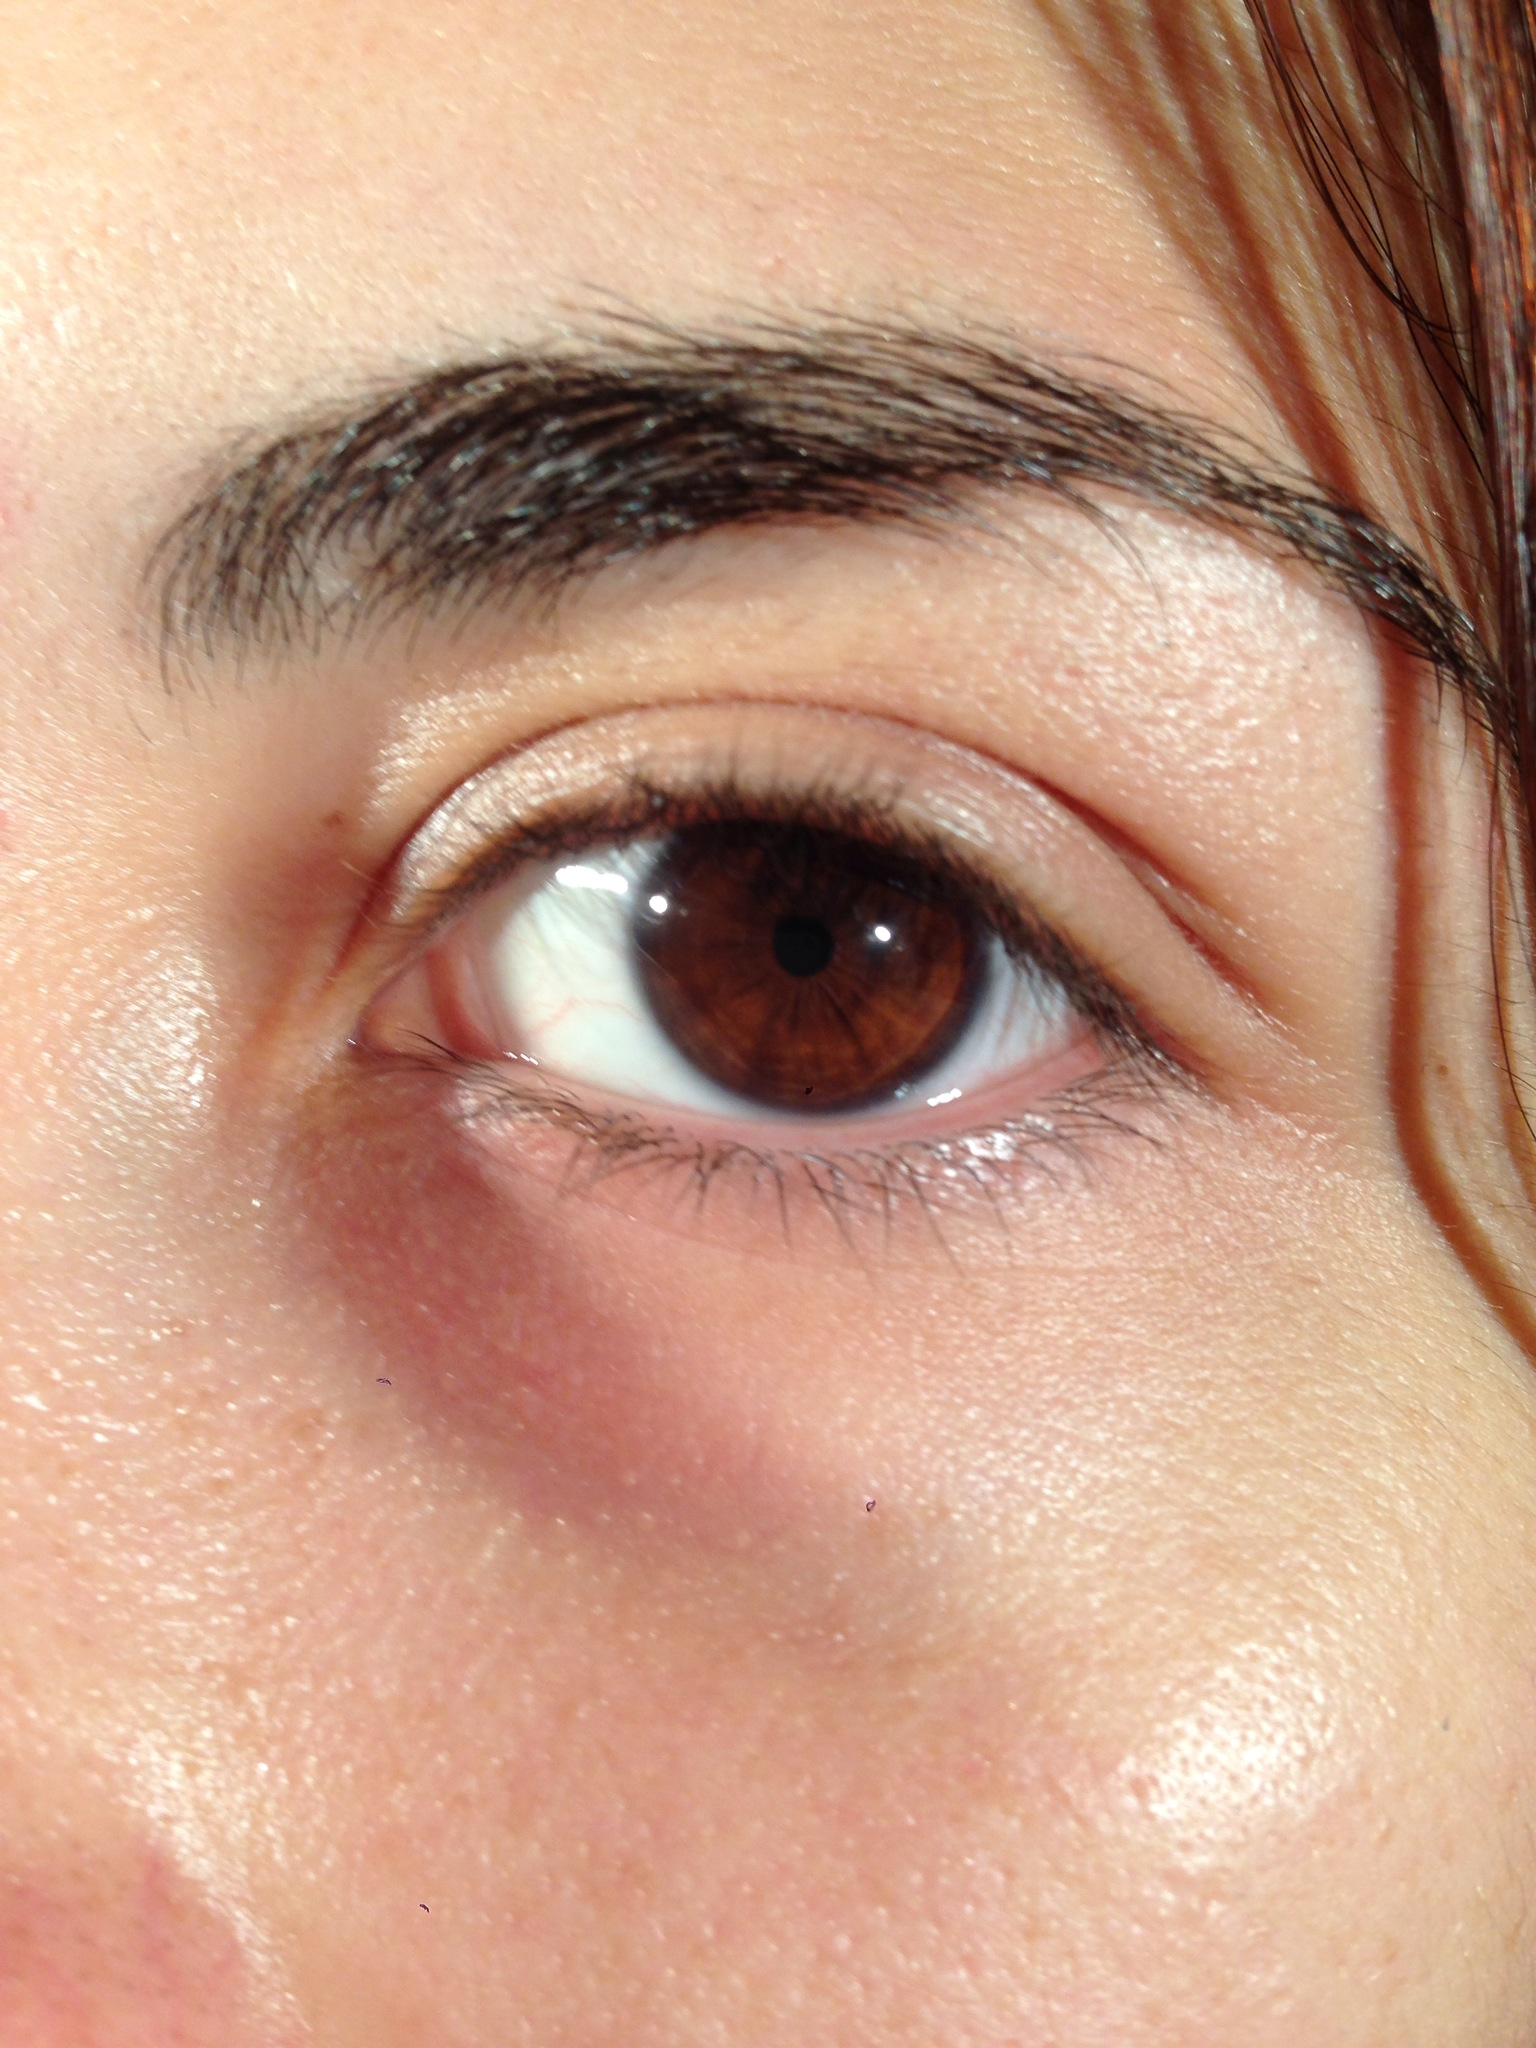
\includegraphics[width=3cm,height=4cm]{img/Resultados/miche/boa_1.jpg}
\end{subfigure}\hfill
\begin{subfigure}{.3\textwidth}
\centering
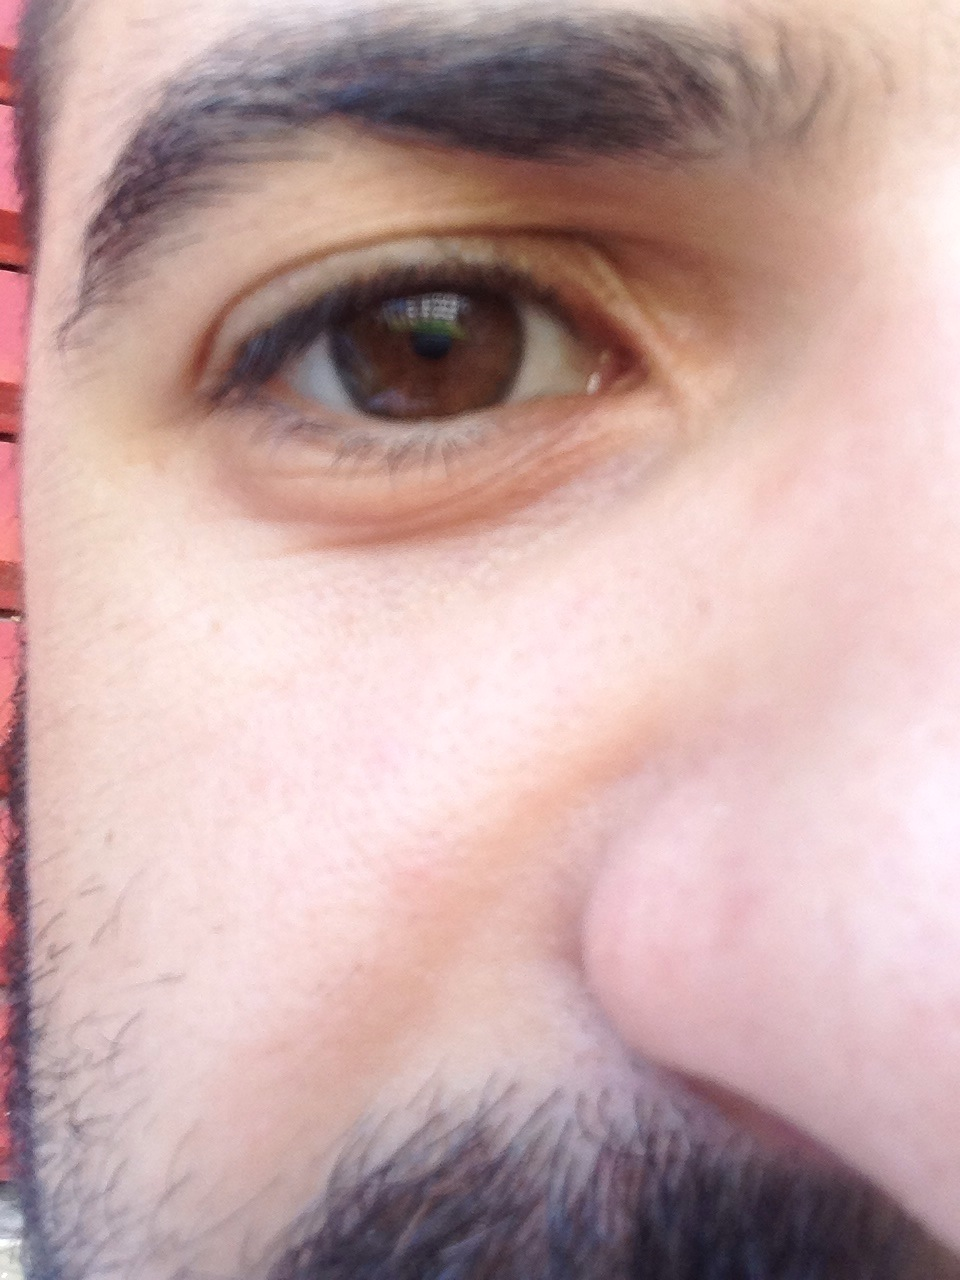
\includegraphics[width=3cm,height=4cm]{img/Resultados/miche/boa_2.jpg}
\end{subfigure}\hfill
\begin{subfigure}{.3\textwidth}
\centering
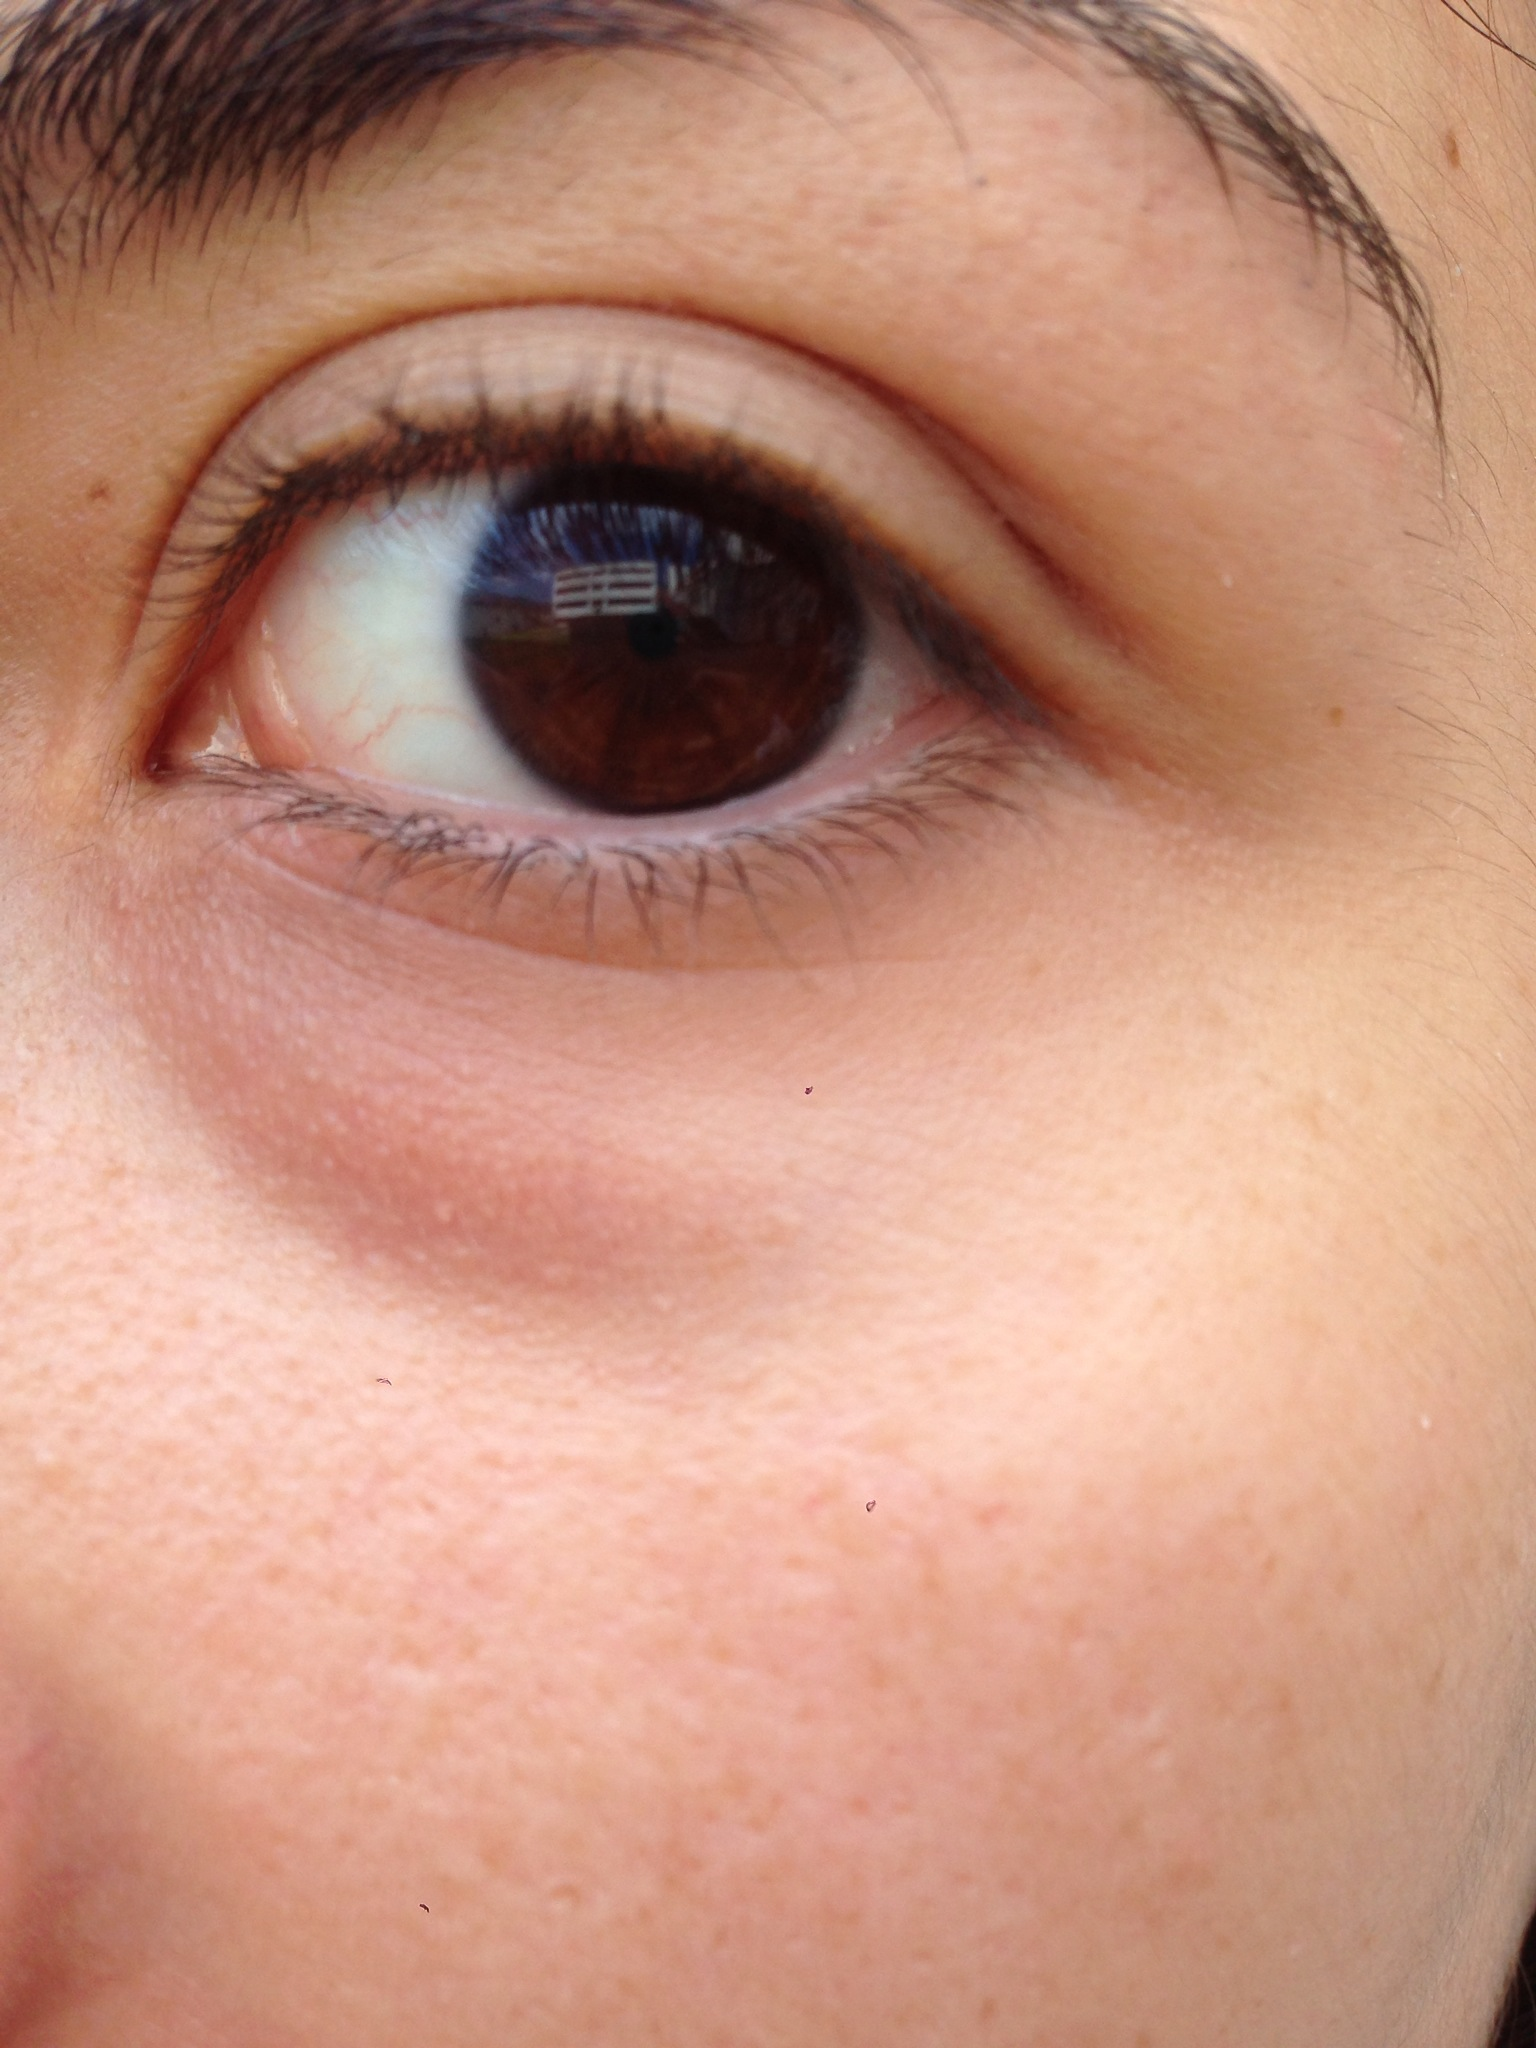
\includegraphics[width=3cm,height=4cm]{img/Resultados/miche/boa_3.jpg}
\end{subfigure}
\caption{Imagens sem a presença de ruídos do \textit{MICHE}.}
\label{fig:experimentos:miche_boas}
\end{figure}

\begin{figure}[h!]
\begin{subfigure}{.3\textwidth}
\centering
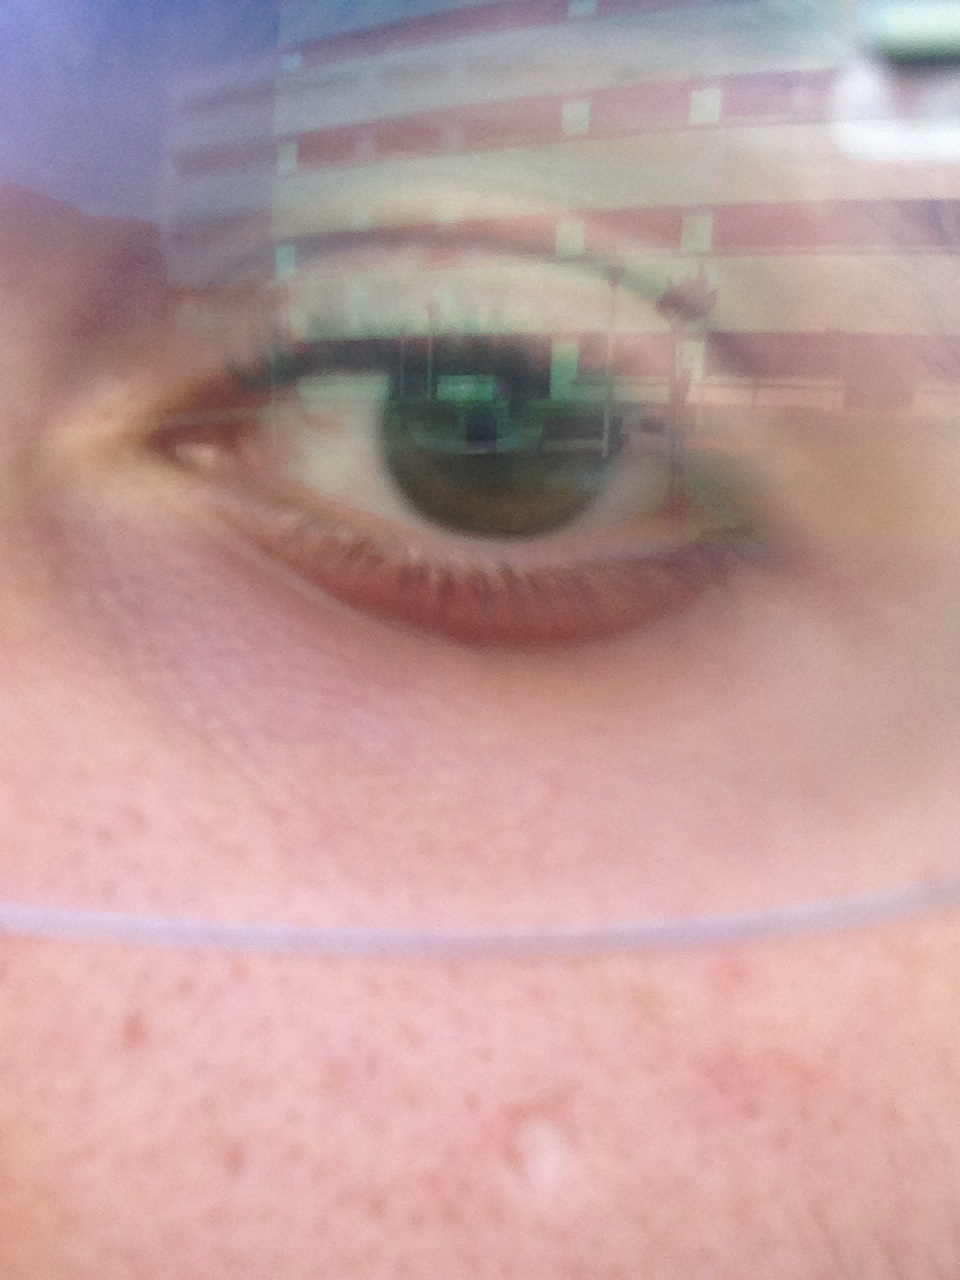
\includegraphics[width=3cm,height=4cm]{img/Resultados/miche/oculos.jpg}
\end{subfigure}\hfill
\begin{subfigure}{.3\textwidth}
\centering
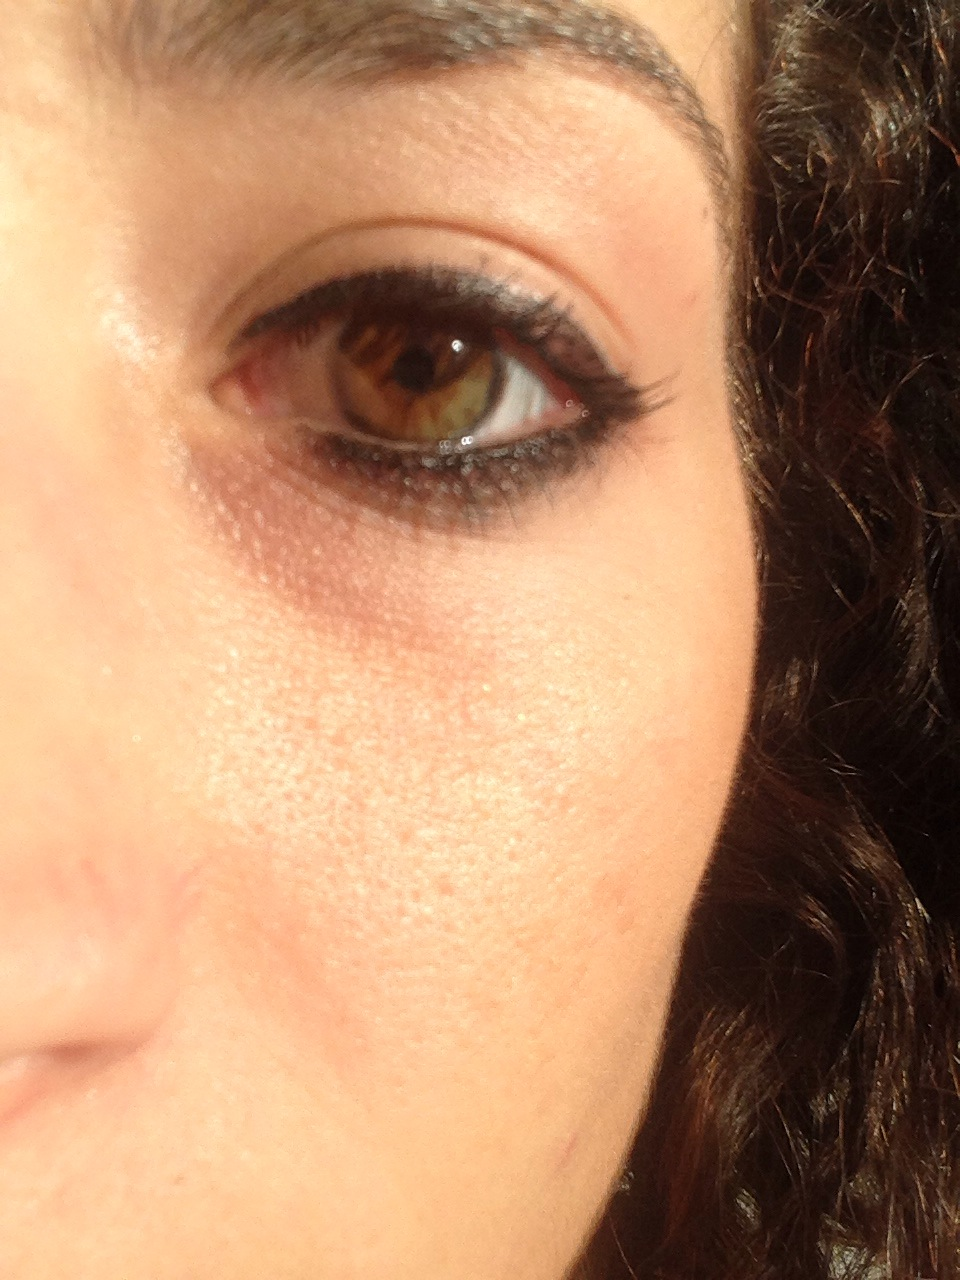
\includegraphics[width=3cm,height=4cm]{img/Resultados/miche/cabelo.jpg}
\end{subfigure}\hfill
\begin{subfigure}{.3\textwidth}
\centering
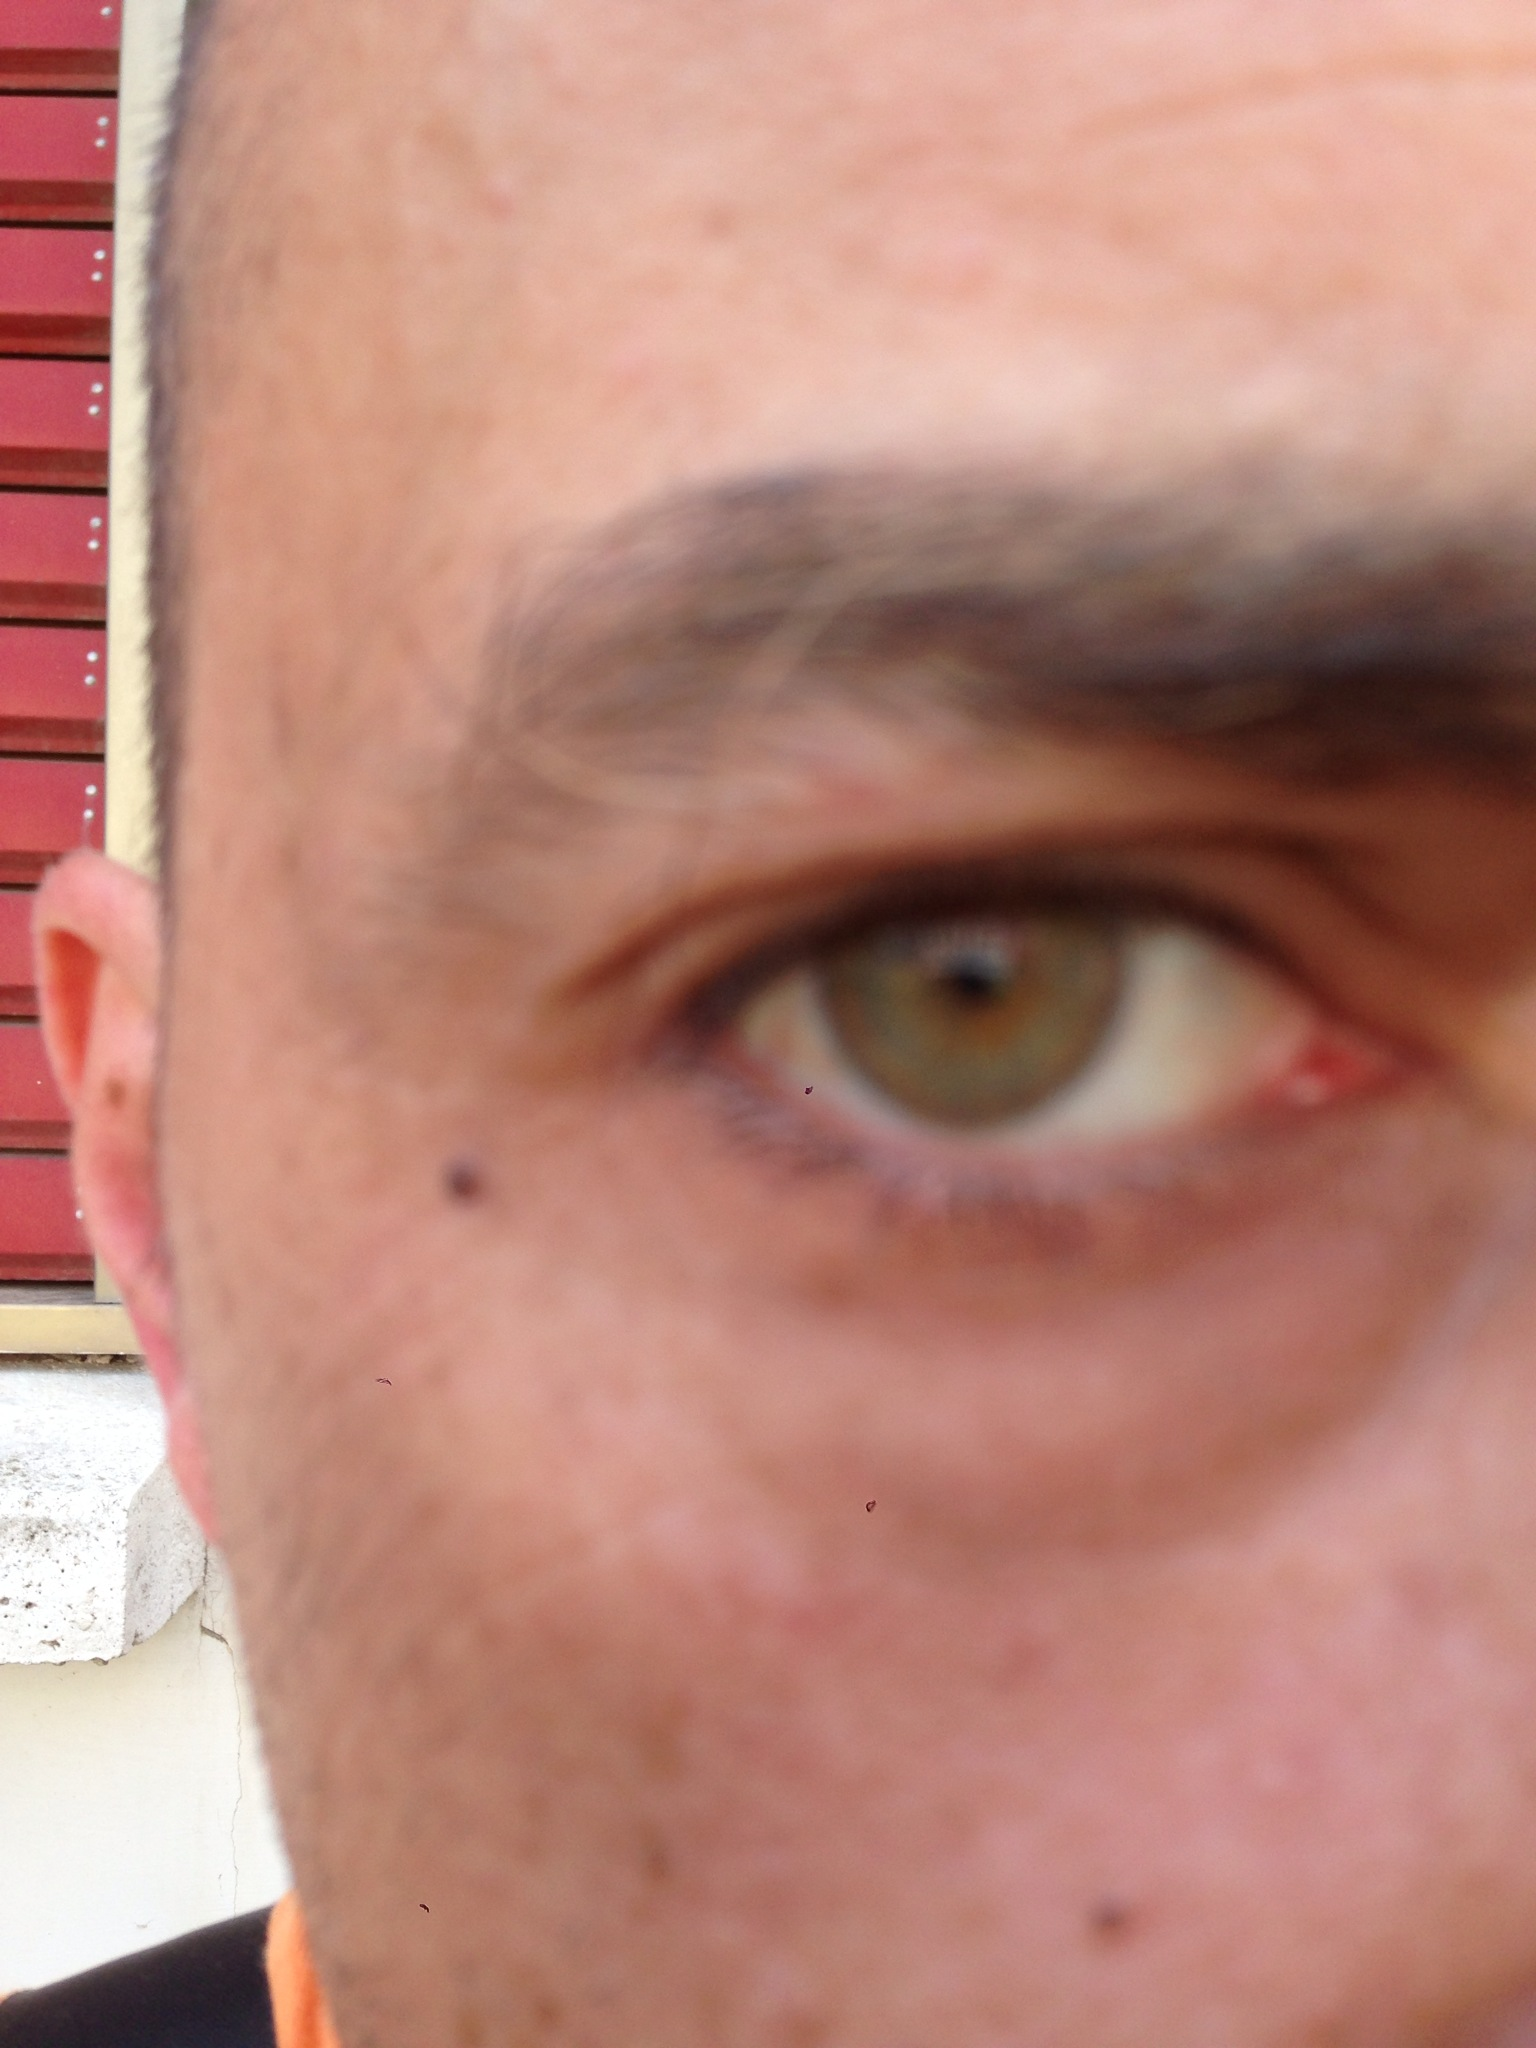
\includegraphics[width=3cm,height=4cm]{img/Resultados/miche/ruidosa_funda.jpg}
\end{subfigure}
\caption{Imagens com distorções do \textit{MICHE}.}
\label{fig:experimentos:miche_ruim}
\end{figure}

\FloatBarrier

\subsection{\textit{UBIRISv1}}\label{sec:experimentos:db:ubirisv1}

\par \textit{UBIRISv1} é um banco de imagens de imagens de íris capturadas por câmera fotográfica com o objetivo de capturar imagens com vários ruídos, de forma a simular ambientes não controlados de aquisição \cite{proenca2005-ubirisv1, ubirisv1}. O banco de imagens possui imagens de 241 indivíduos, totalizando 1877 imagens. As imagens são capturadas pela câmera \textit{Nikon E5700} e foram tiradas em duas sessões, onde:

\begin{itemize}
    \item Primeira sessão: Imagens foram capturadas com o objetivo de minimizar ruídos, como reflexo, luminosidade e contraste, e a estrutura para capturar as imagens foi montada em uma sala sem a presença de luz natural;
    \item Segunda sessão: Local de captura foi mudado, para incorporar fatores de luminosidade natural, de forma que ruídos como reflexos, problemas de foco, contraste aparecem nas imagens.
\end{itemize}

\par Neste projeto, foram separadas imagens de 20 indivíduos da primeira sessão e 20 da segunda sessão.

\par As Figuras \ref{fig:experimentos:ubirisv1_sessao1} e \ref{fig:experimentos:ubirisv1_sessao2} ilustram imagens capturadas na primeira e segunda sessão dos mesmos indivíduos, respectivamente.

\begin{figure}[h!]
\begin{subfigure}{.3\textwidth}
\centering
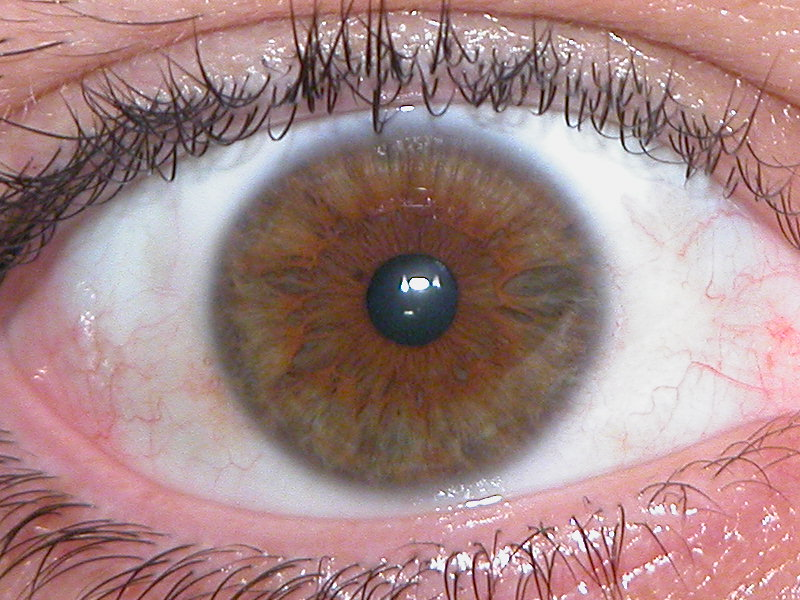
\includegraphics[width=4cm,height=3.5cm]{img/Resultados/ubirisv1/sessao1_1.jpg}
\end{subfigure}\hfill
\begin{subfigure}{.3\textwidth}
\centering
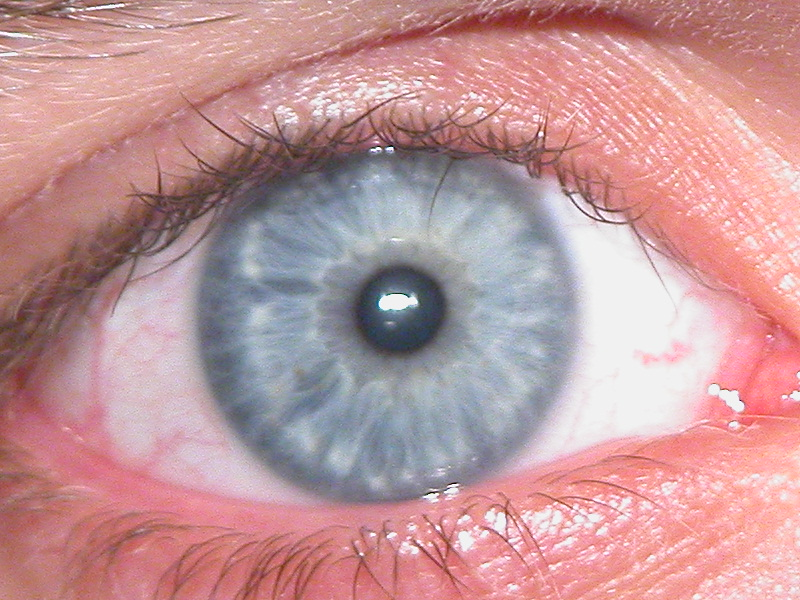
\includegraphics[width=4cm,height=3.5cm]{img/Resultados/ubirisv1/sessao1_55.jpg}
\end{subfigure}\hfill
\begin{subfigure}{.3\textwidth}
\centering
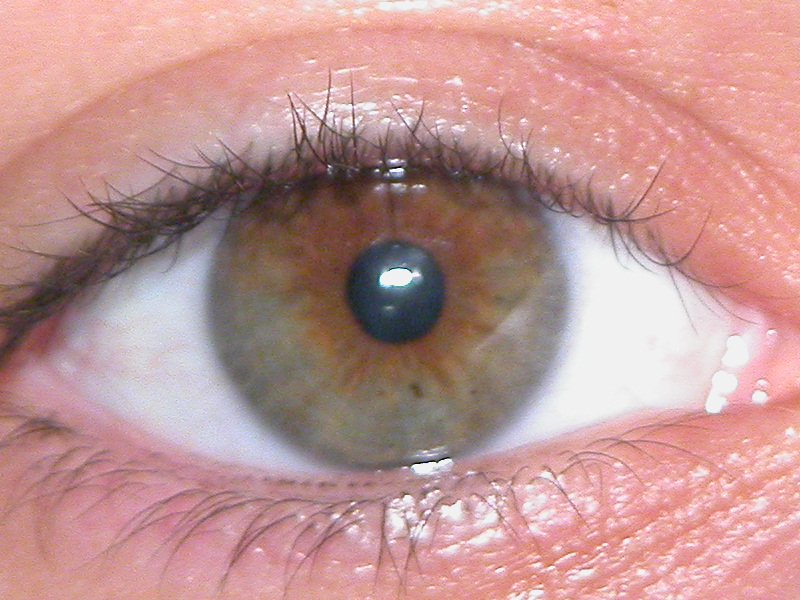
\includegraphics[width=4cm,height=3.5cm]{img/Resultados/ubirisv1/sessao1_76.jpg}
\end{subfigure}
\caption{Imagens da primeira sessão do \textit{UBIRISv1}.}
\label{fig:experimentos:ubirisv1_sessao1}
\end{figure}

\begin{figure}[h!]
\begin{subfigure}{.3\textwidth}
\centering
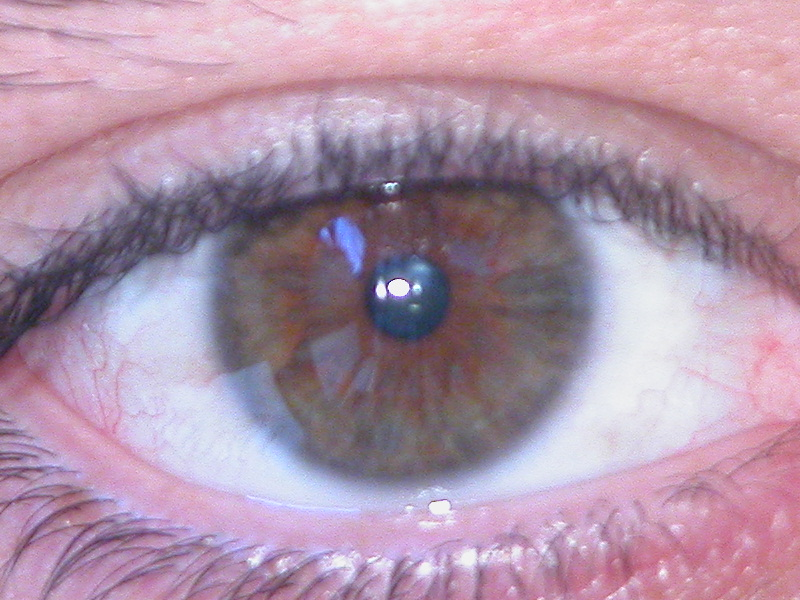
\includegraphics[width=4cm,height=3.5cm]{img/Resultados/ubirisv1/sessao2_1.jpg}
\end{subfigure}\hfill
\begin{subfigure}{.3\textwidth}
\centering
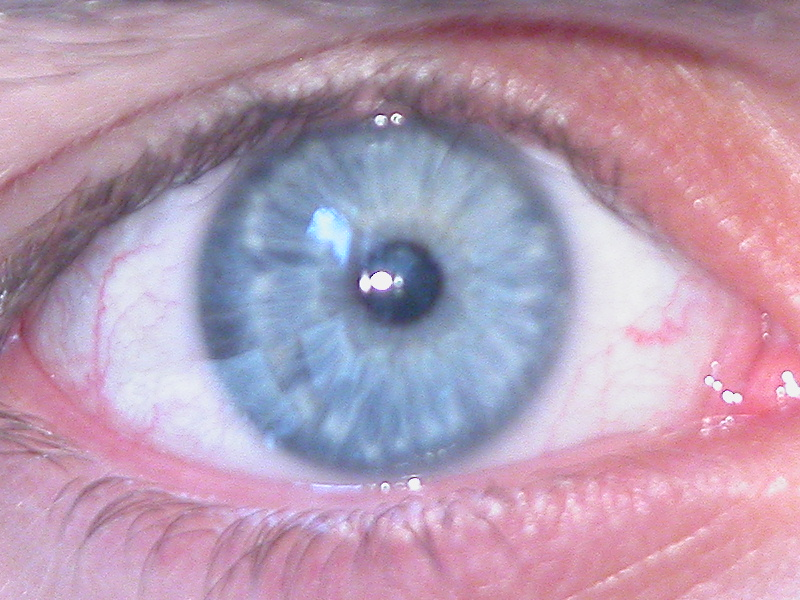
\includegraphics[width=4cm,height=3.5cm]{img/Resultados/ubirisv1/sessao2_55.jpg}
\end{subfigure}\hfill
\begin{subfigure}{.3\textwidth}
\centering
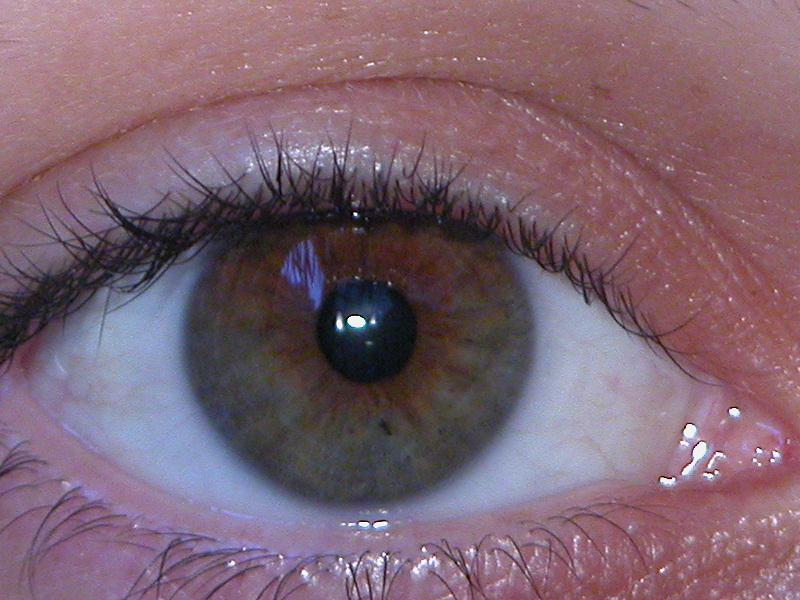
\includegraphics[width=4cm,height=3.5cm]{img/Resultados/ubirisv1/sessao2_76.jpg}
\end{subfigure}
\caption{Imagens da segunda sessão do \textit{UBIRISv1}.}
\label{fig:experimentos:ubirisv1_sessao2}
\end{figure}

\FloatBarrier

\subsection{\textit{UBIRISv2}}\label{sec:experimentos:db:ubirisv2}

\par \textit{UBIRISv2} é um banco de imagens de imagens de íris dos mesmos autores do \textit{UBIRISv1}, com o objetivo de deixar as imagens mais realistas, ou seja, com mais tipos de ruídos e em diversas distâncias \cite{proence2010-ubirisv2}. O banco de imagens é composto por 11102 imagens distribuídas em 261 indivíduos. As imagens foram capturadas pela câmera \textit{Canon EOS 5D}.

\par A captura de imagens foi dividida em duas sessões, onde somente a localização da câmera e o tipo de luz artificial no ambiente mudaram. Três imagens são capturadas em cinco distâncias diferentes da câmera, entre 4 e 8 metros, totalizando 15 imagens por indivíduo em cada sessão: 

\begin{itemize}
    \item 8 metros: I1-I3;
    \item 7 metros: I4-I6;
    \item 6 metros: I7-I9;
    \item 5 metros: I10-I12;
    \item 4 metros: I13-I15.
\end{itemize}

\par Foi solicitado aos indivíduos que olhassem para pontos diferentes no ambiente enquanto andavam lentamente entre as marcas das distância, de forma a capturar imagens da íris em ângulos diferentes e em movimento para introduzir ruídos.

\par No projeto, foram utilizadas somente imagens da primeira sessão do banco de imagens e imagens capturadas a 4 e 5 metros da câmera (I11-I15), por conta de algumas restrições dos parâmetros de tamanho mínimo e máximo da pupila e íris do algoritmo de segmentação do sistema \textit{OSIRISv4.1}.

\par A \refFig{fig:experimentos:ubirisv2} ilustra exemplos de imagens das cinco distâncias usadas do \textit{UBIRISv2}.

\begin{figure}[htb]
    \centering % <-- added
\begin{subfigure}{0.25\textwidth}
  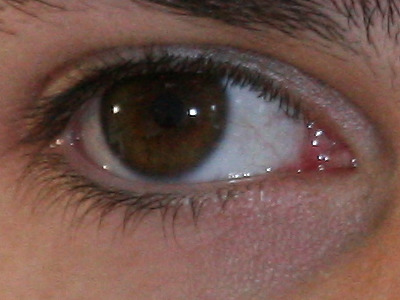
\includegraphics[width=\linewidth]{img/Resultados/ubirisv2/C3_S1_I11.jpg}
  \caption{I11.}
\end{subfigure}\hfil % <-- added
\begin{subfigure}{0.25\textwidth}
  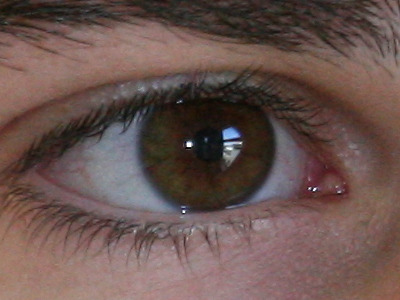
\includegraphics[width=\linewidth]{img/Resultados/ubirisv2/C3_S1_I12.jpg}
  \caption{I12.}
  \label{fig:2}
\end{subfigure}\hfil % <-- added
\begin{subfigure}{0.25\textwidth}
  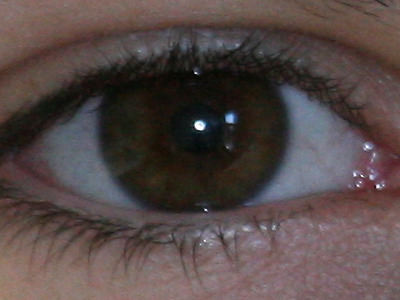
\includegraphics[width=\linewidth]{img/Resultados/ubirisv2/C3_S1_I13.jpg}
  \caption{I13.}
\end{subfigure}

\medskip
\begin{subfigure}{0.25\textwidth}
  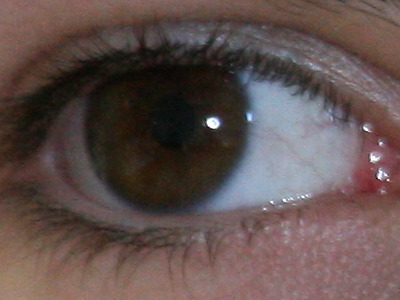
\includegraphics[width=\linewidth]{img/Resultados/ubirisv2/C3_S1_I14.jpg}
  \caption{I14.}
\end{subfigure}\hfil % <-- added
\begin{subfigure}{0.25\textwidth}
  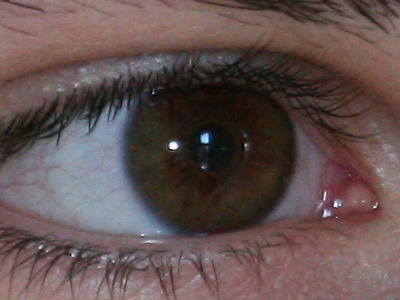
\includegraphics[width=\linewidth]{img/Resultados/ubirisv2/C3_S1_I15.jpg}
  \caption{I15.}
\end{subfigure}\hfil % <-- added
\caption{Imagens do banco de imagens \textit{UBIRISv2} capturadas a 5 e 4 metros da câmera.}
\label{fig:experimentos:ubirisv2}
\end{figure}

\FloatBarrier

\subsection{\textit{\acrshort{Warsaw}}}\label{sec:experimentos:db:warsaw}

\par \textit{\acrshort{Warsaw}} é um banco de imagens de imagens de íris capturadas por \textit{smartphones} \cite{trokielwicz2016-Warsaw}. Tem o objetivo de propor imagens de íris de \textit{smartphones} de boa qualidade e avaliar seu rendimento em sistemas de reconhecimento de íris conhecidos. Participaram do projeto 70 voluntários, em que a captura das imagens de suas íris esquerda e direita foi dividida em duas sessões e em ambientes fechados. As imagens foram capturadas pelo \textit{smartphone} \textit{iPhone 5s} e em todas, foi utilizada a câmera traseira com \textit{flash}. No total, foram capturadas 3192 imagens de 139 íris esquerdas e 136 íris direitas dos 70 voluntários.

\par No projeto, foram utilizadas somente imagens da primeira sessão e os olhos foram selecionados alternadamente entre os indivíduos. Imagens da segunda sessão não foram utilizadas porque nem todos os indivíduos que participaram da primeira sessão participaram da segunda e em muitos casos, cada indivíduo só possuia de duas a quatro imagens por olho, quantidade insuficiente para os experimentos.

\par A \refFig{fig:experimentos:warsaw_1} ilustra imagens da primeira sessão do banco de imagens \textit{\acrshort{Warsaw}}.

\begin{figure}[H]
    \centering % <-- added
\begin{subfigure}{0.25\textwidth}
  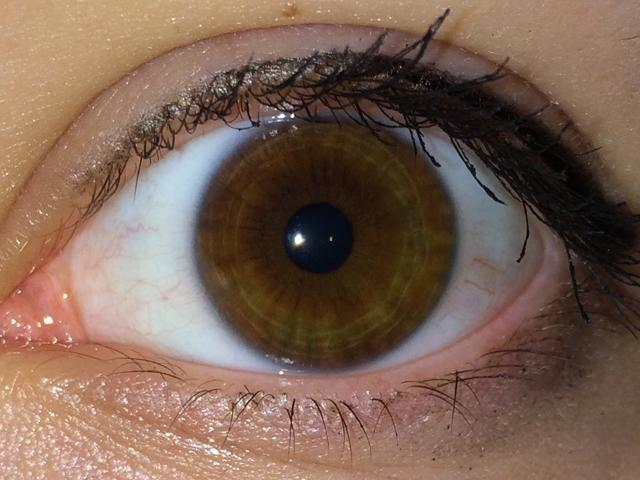
\includegraphics[width=\linewidth]{img/Resultados/warsaw/left_1.jpg}
  \caption{}
\end{subfigure}\hfil % <-- added
\begin{subfigure}{0.25\textwidth}
  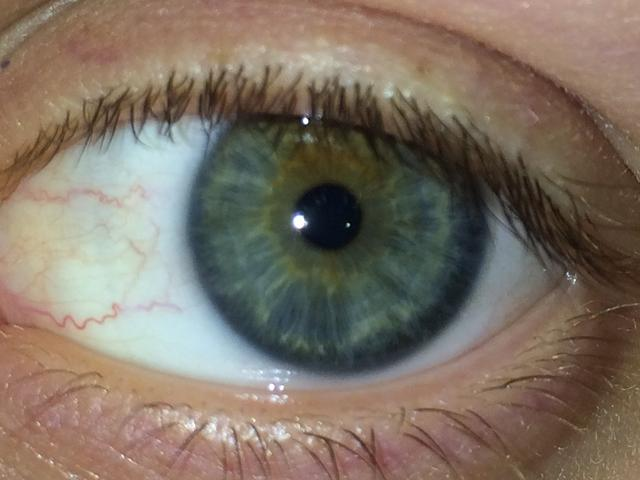
\includegraphics[width=\linewidth]{img/Resultados/warsaw/left_17.jpg}
  \caption{}
\end{subfigure}\hfil % <-- added
\begin{subfigure}{0.25\textwidth}
  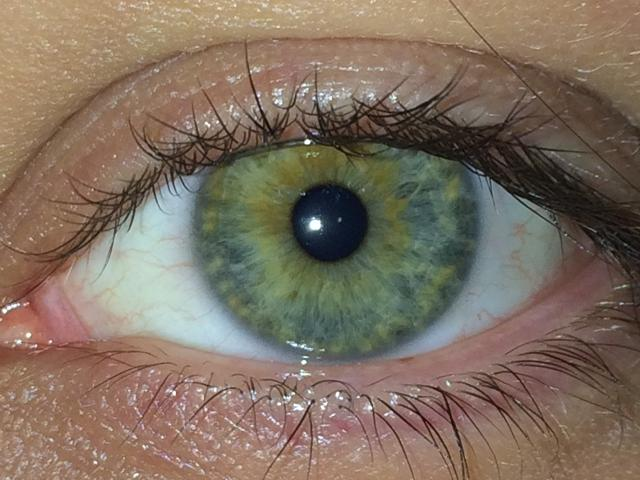
\includegraphics[width=\linewidth]{img/Resultados/warsaw/left_65.jpg}
  \caption{}
\end{subfigure}

\medskip
\begin{subfigure}{0.25\textwidth}
  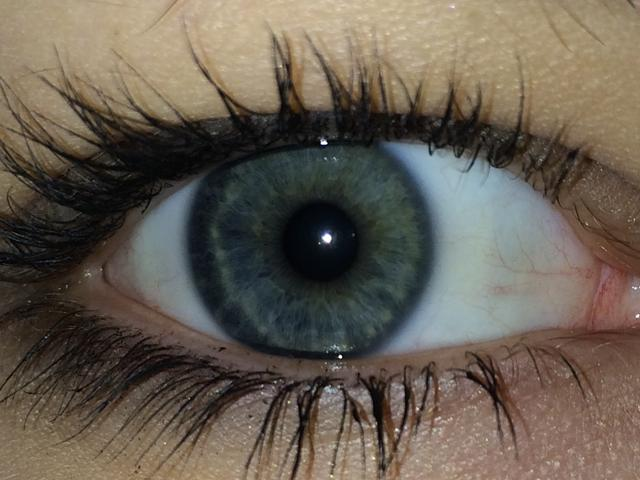
\includegraphics[width=\linewidth]{img/Resultados/warsaw/right_22.jpg}
  \caption{}
\end{subfigure}\hfil % <-- added
\begin{subfigure}{0.25\textwidth}
  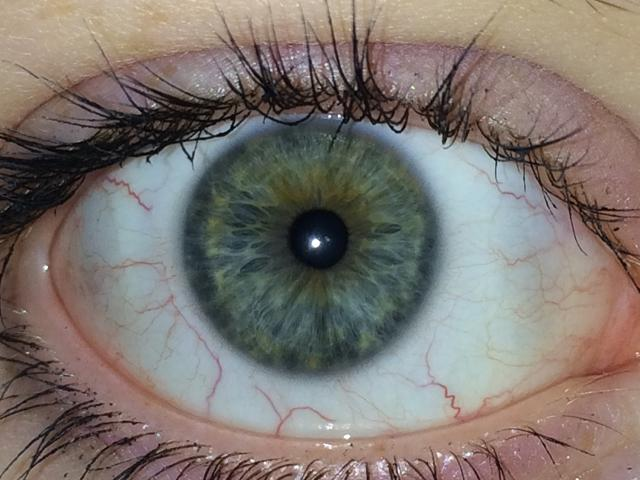
\includegraphics[width=\linewidth]{img/Resultados/warsaw/right_32.jpg}
  \caption{}
\end{subfigure}\hfil % <-- added
\begin{subfigure}{0.25\textwidth}
  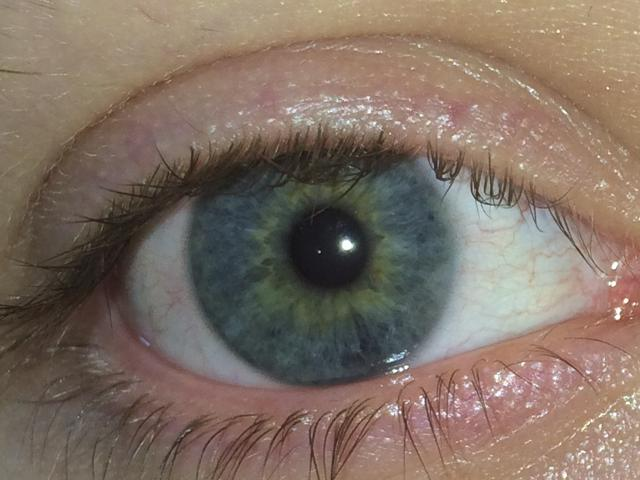
\includegraphics[width=\linewidth]{img/Resultados/warsaw/right_68.jpg}
  \caption{}
\end{subfigure}
\caption{As imagens (a)-(c) ilustram olhos esquerdos e (d)-(f) olhos direitos da primeira sessão do \textit{\acrshort{Warsaw}} de pessoas diferentes.}
\label{fig:experimentos:warsaw_1}
\end{figure}

\FloatBarrier

\subsection{Limiares $T_{DSMI}$ e $T_{FCE}$} \label{sec:experimentos:db:limiares}

\par Como os banco de imagens escolhidos para os experimentos possuem características diferentes, os limiares $T_{DSMI}$ e $T_{FCE}$ da arquitetura proposta (\refFig{fig:metodologia:arquitetura}) foram calculados separadamente para cada banco de imagens.

\par Para calcular o limiar $T_{DSMI}$ foram usadas as duas imagens de treino de 40 indivíduos dos bancos de imagens, totalizando 80 por banco de imagens. As etapas para o cálculo do limiar de cada banco de imagens são enumeradas abaixo:

\begin{enumerate}
    \item Calcular a métrica de qualidade \textit{\acrshort{DSMI}} das 80 imagens;
    \item Gerar o histograma das métricas calculadas;
    \item O limiar $T_{DSMI}$ consiste no limiar \textit{Otsu} (Seção \ref{sec:dom_esp:otsu}) calculado a partir do histograma.
\end{enumerate}

\par O cálculo do limiar $T_{FCE}$ seguiu os mesmos passos descritos para o limiar $T_{DSMI}$, mas antes foram executadas as etapas de segmentação do \textit{OSIRISv4.1} das 80 imagens de cada banco de imagens e ao invés de calcular a qualidade das imagens de íris usando a métrica \textit{\acrshort{DSMI}}, foram calculadas as qualidades das segmentações pela métrica de qualidade \textit{\acrshort{FCE}}. Os limiares calculados para cada banco de imagens são mostrados na \refTab{tab:experimentos:limiares_dsmi_fce}.

\begin{table}[H]
\centering
\captionof{table}{Valores dos limiares $T_{DSMI}$ e $T_{FCE}$ calculados para todos os bancos de imagens.} \label{tab:experimentos:limiares_dsmi_fce} 
\begin{tabular}{lllll}
\cline{2-5}
\multicolumn{1}{l|}{}             & \multicolumn{1}{l|}{\textit{\textbf{MICHE}}} & \multicolumn{1}{l|}{\textit{\textbf{UBIRISv1}}} & \multicolumn{1}{l|}{\textit{\textbf{UBIRISv2}}} & \multicolumn{1}{l|}{\textit{\begin{tabular}[c]{@{}l@{}}\textbf{Warsaw}\end{tabular}}} \\ \hline
\multicolumn{1}{|l|}{\textit{\textbf{$T_{DSMI}$}}} & \multicolumn{1}{l|}{0.75}           & \multicolumn{1}{l|}{0.83}              & \multicolumn{1}{l|}{0.69}              & \multicolumn{1}{l|}{0.51}                                                                                    \\ \hline
\multicolumn{1}{|l|}{\textit{\textbf{$T_{FCE}$}}} & \multicolumn{1}{l|}{0.54}           & \multicolumn{1}{l|}{0.85}              & \multicolumn{1}{l|}{0.54}              & \multicolumn{1}{l|}{0.9}                                                                                     \\ \hline
                                  &                                     &                                        &                                        &                                                                                                 
\end{tabular}
\end{table}

\par O limiar de \textit{Otsu} calcula o limiar que maximiza a variância entre duas classes (Seção \ref{sec:dom_esp:otsu}). Pela \refTab{tab:experimentos:limiares_dsmi_fce}, é possível notar como os valores encontrados para os dois limiares variaram para cada banco de imagens. O valor do limiar $T_{DSMI}$  do \textit{MICHE} é elevado, apesar de alguns ruídos presentes nas imagens e o valor do limiar $T_{FCE}$ é baixo, porque as imagens foram incorretamente segmentadas pelo algoritmo de segmentação do \textit{OSIRISv4.1}, que apresentou deficiências. Os limiares do banco de imagens \textit{UBIRISv1} apresentaram valores condizentes, porque suas imagens são capturadas em condições apropriadas e controladas, e as íris foram corretamente segmentadas. O banco de imagens \textit{UBIRISv2}, assim como o \textit{MICHE}, é desafiador, porque as imagens apresentam ruídos e causam dificuldades para a segmentação, por conta das diferenças de distância que as imagens foram capturadas, como explicado na Seção \ref{sec:experimentos:db:ubirisv2}, e apresentou valores de limiares esperados para suas condições. O limiar $T_{DSMI}$ calculado para o banco de imagens \textit{\acrshort{Warsaw}} pode ser considerado baixo, mas é o que melhor separa as qualidades da métrica \textit{\acrshort{DSMI}} calculadas das imagens do banco de imagens e o limiar $T_{FCE}$ apresentou um valor condizente, já que as imagens, no geral, tiveram suas íris corretamente segmentadas.


% O banco de imagens \textit{\acrshort{Warsaw}} foi o que apresentou o resultado menos esperado para o limiar $T_{DSMI}$, porque as suas imagens, analisando subjetivamente, são muito boas, como ilustrado nas Figuras \ref{fig:experimentos:warsaw_1} e \ref{fig:experimentos:warsaw_2}, e nãoque o valor do limiar $T_{FCE}$ foi esperado, porque as segmentações apresentaram bons resultados.

\FloatBarrier

\subsection{Ruídos} \label{sec:experimentos:ruidos}

\par Conforme explicado na Seção \ref{sec:experimentos:db}, cinco imagens de 40 indivíduos foram escolhidas aleatoriamente em todos os bancos de imagens. Dessas cinco imagens, duas foram reservadas para o cálculo dos limiares $T_{DSMI}$ e $T_{FCE}$ e três para a análise do desempenho da arquitetura de sistema de reconhecimento de íris proposta usando as métricas \textit{\acrshort{DSMI}} e \textit{\acrshort{FCE}}. 

\par Como a qualidade das imagens podem influenciar diretamente na segmentação de íris e três imagens de teste serem muito poucas para os experimentos, por conta da limitação que os bancos de imagens impuseram, foram geradas imagens com seis ruídos artificiais: \textit{Desfoque Gaussiano}, \textit{Impulso (Sal e Pimenta)}, \textit{\acrfull{WGN}}, \textit{Superexposição}, \textit{Desfoque Móvel} e o padrão de compressão \textit{JPEG2000}. Os cinco primeiros ruídos foram escolhidos porque são os ruídos mais comuns em imagens de íris e são utilizados nos experimentos da métrica \textit{\acrshort{DSMI}} \cite{Jenadeleh_2018_CVPR_Workshops} e o padrão de compressão \textit{JPEG2000} é a utilizada nos experimentos da métrica \textit{\acrshort{FCE}} \cite{du2010}. Para cada ruído, são usados quatro parâmetros diferentes, de forma que são geradas quatro imagens ruidosas. Os ruídos são gerados para cada imagem de teste, de forma que para cada, 24 novas imagens são geradas e no final, totalizam 3000 imagens para serem usadas nos experimentos em cada banco de imagens.  A \refTab{tab:experimentos:ruidos} lista os ruídos com os parâmetros utilizados para gerá-los, em que neste projeto foi utilizado a linguagem de programação \textit{MATLAB}. A \refFig{fig:experimentos:ruidos} ilustra exemplos de imagens de íris com os ruídos gerados.

% \par Ruídos em imagens digitais são distorções causadas por variações aleatórias no brilho ou cor das imagens, podem ser causados por fatores como o sensor da câmera, iluminação, desfoque, compressão e diminuem a qualidade das imagens \cite{gonsalez2006}. O ruído \textit{Desfoque Gaussiano} consiste em ruídos causados pela função \textit{Gaussiana} e causam suavizações nas imagens \cite{gonsalez2006, boyat2015review}. O ruído de Impulso \textit{Sal e Pimenta} consiste em distúrbios no sinal da imagem que provocam \textit{pixels} brancos e pretos distribuídos na imagem \cite{gonsalez2006, boyat2015review}. O ruído \textit{\acrshort{WGN}} consiste em um ruído causado por sinais aleatórios com intensidades uniformes em frequências que seguem a distribuição \textit{Gaussiana} e causam distorções distribuídas na imagem \cite{boyat2015review}. \textit{Superexposição} é um ruído causado por muita iluminação na hora da captura de imagens e faz com que as intensidades dos \textit{pixels} das imagens tenham valores elevados \cite{overexposure}. \textit{Desfoque Móvel} é o ruído causado por movimento da câmera sendo usada para capturar alguma imagem, no movimento do objeto ou paisagem sendo capturada pela câmera, e causam desfoques na imagem \cite{jiang2005motion}. O padrão de compressão com perdas \textit{JPEG2000} consiste na utilização de técnicas para reduzir o tamanho da imagem, podendo perder a sua qualidade original, e quanto maior a taxa de compressão escolhida, mais distorções são inseridas na imagem resultante \cite{marcellin2000-jpeg2000}. A \refTab{tab:experimentos:ruidos} lista os ruídos descritos acima com os parâmetros utilizados para gerá-los.

\begin{table}[h!]
\centering
\caption{Ruídos gerados e os parâmetros utilizados}
\label{tab:experimentos:ruidos}
\begin{tabular}{|l|l|}
\hline
\multicolumn{1}{|c|}{\textbf{Ruídos}} & \multicolumn{1}{c|}{\textbf{Parâmetros}} \\ \hline
\textit{Desfoque Gaussiano} & {}$\sigma$ = 0.5, 2, 3.5, 5 {} \\ \hline
\textit{Impulso (Sal e Pimenta)} & {}Densidade = 0.05, 0.2, 0.35, 0.5 {} \\ \hline
\textit{\acrshort{WGN}} & {}$\mu = 0$; $\sigma^2$ = 0.002, 0.008, 0.014, 0.02{} \\ \hline
\textit{Superexposição} & {}Constante = 10, 40, 70, 100 {} \\ \hline
\textit{Desfoque Móvel} & {}Comprimento, $\theta$ = 10, 26.66, 43.33, 60{} \\ \hline
\textit{JPEG2000} & {}Taxa de compressão = 25, 50, 75, 100{} \\ \hline
\end{tabular}
\end{table}

% \par A \refFig{fig:experimentos:ruidos} ilustra exemplos de imagens de íris com os ruídos gerados.

\begin{figure}[H]
\centering
\begin{subfigure}{0.25\textwidth}
  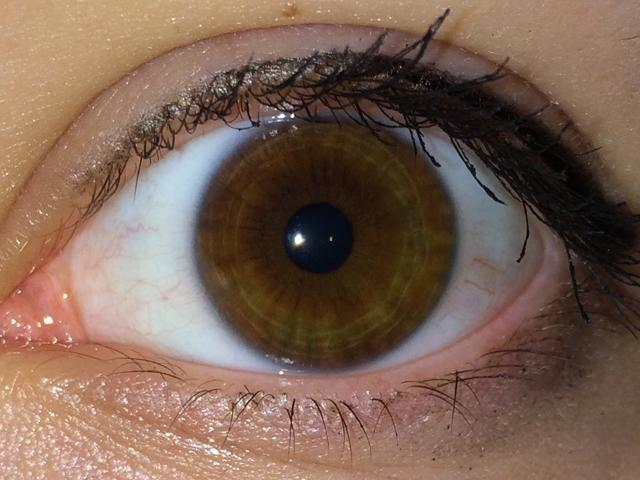
\includegraphics[width=\linewidth]{img/Resultados/ruidos/original.jpg}
  \caption{Imagem original.}
\end{subfigure}\vfil
\centering % <-- added
\begin{subfigure}{0.25\textwidth}
  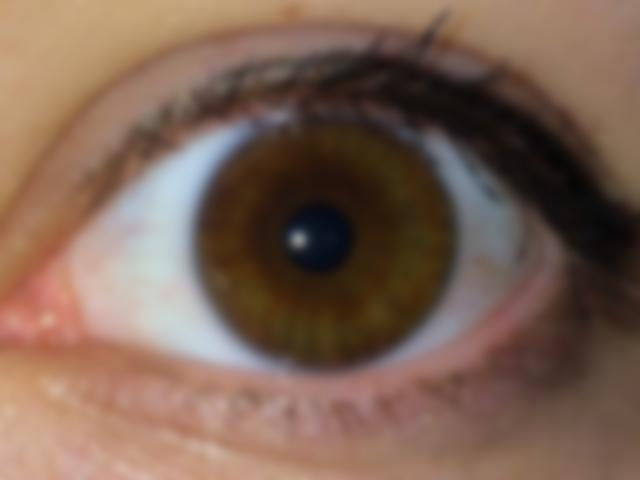
\includegraphics[width=\linewidth]{img/Resultados/ruidos/gaussian5.jpg}
  \caption{\textit{Desfoque Gaussiano}, $\sigma=5$.}
\end{subfigure}\hfil % <-- added
\begin{subfigure}{0.25\textwidth}
  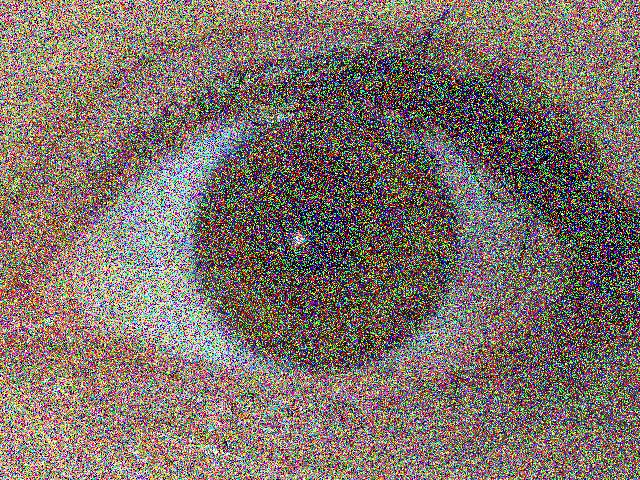
\includegraphics[width=\linewidth]{img/Resultados/ruidos/impulse0,5.jpg}
  \caption{\textit{Sal e Pimenta}, Densidade = 0.5.}
\end{subfigure}\hfil % <-- added
\begin{subfigure}{0.25\textwidth}
  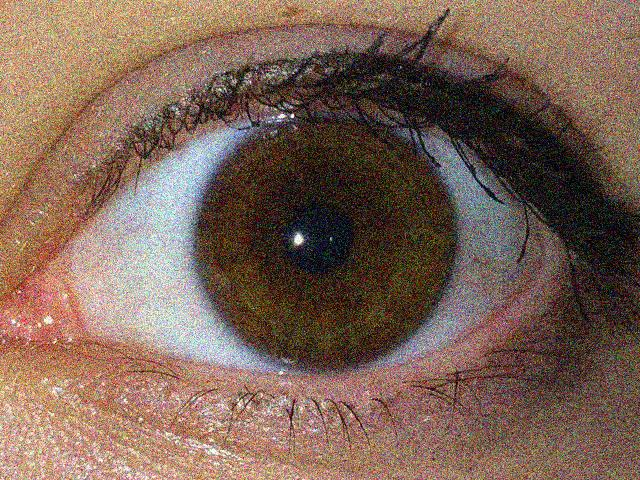
\includegraphics[width=\linewidth]{img/Resultados/ruidos/wgn0,02.jpg}
  \caption{\textit{\acrshort{WGN}}, $\sigma^2 = 0.02$.}
\end{subfigure}

\medskip
\begin{subfigure}{0.25\textwidth}
  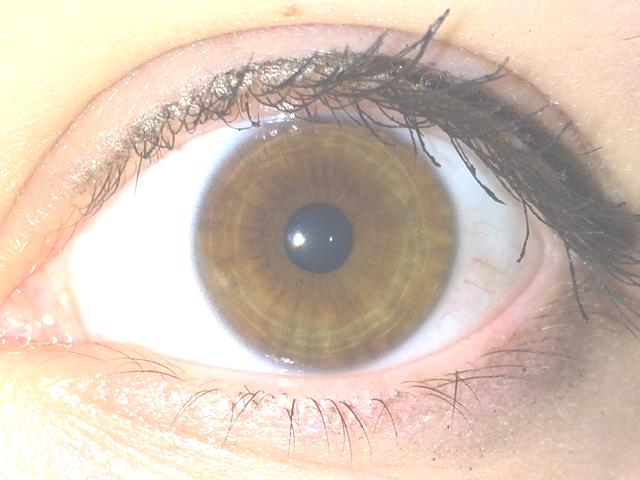
\includegraphics[width=\linewidth]{img/Resultados/ruidos/over_exposure100.jpg}
  \caption{\textit{Superexposição}, Constante = 100.}
\end{subfigure}\hfil % <-- added
\begin{subfigure}{0.25\textwidth}
  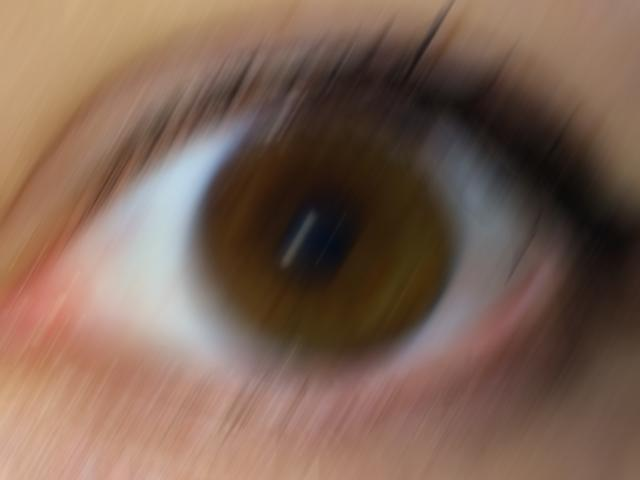
\includegraphics[width=\linewidth]{img/Resultados/ruidos/motion_blur60.jpg}
  \caption{\textit{Desfoque móvel}, Comprimento e $\theta$ = 60.}
\end{subfigure}\hfil % <-- added
\begin{subfigure}{0.25\textwidth}
  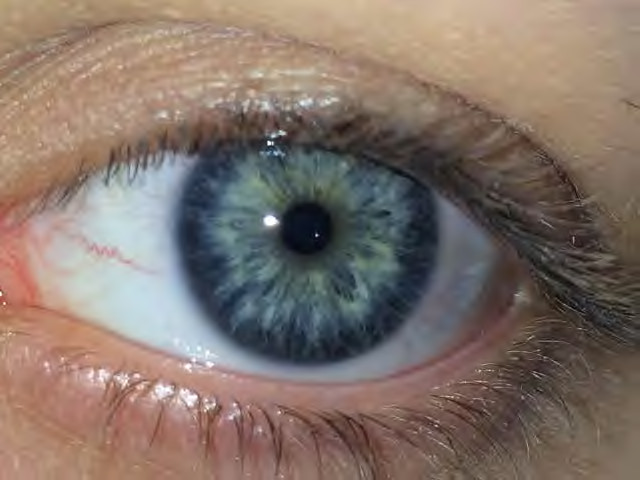
\includegraphics[width=\linewidth]{img/Resultados/ruidos/jpeg2000_100.jpg}
  \caption{\textit{JPEG2000}, Taxa de compressão = 100.}
\end{subfigure}
\caption{Imagem original e imagens resultantes para cada ruído.}
\label{fig:experimentos:ruidos}
\end{figure}

\FloatBarrier

\section{Segmentação} \label{sec:experimentos:segmentacao}

% \par A segmentação é a etapa mais importante de um sistema de reconhecimento de íris, porque da íris segmentada que são extraídos os atributos necessários para sua codificação, de forma que identificam unicamente um indivíduo. Neste projeto, o objetivo é a análise das duas métricas de qualidade, \textit{\acrshort{DSMI}} e \textit{\acrshort{FCE}}, no rendimento de sistemas de reconhecimento de íris e, como explicado na Seção \ref{sec:metodologia:arquitetura}, foi escolhido o sistema de reconhecimento de íris \textit{OSIRISv4.1}. 

\par O algoritmo de segmentação do \textit{OSIRISv4.1} consiste em encontrar primeiro a pupila e depois encontrar os contornos da íris com base em intervalos de valores para os raios, como explicado na Seção \ref{sec:metodologia:segmentacao}. Em seus arquivos de configuração, devem ser passados quatro argumentos: diâmetros mínimos e máximos da pupila e íris. Os parâmetros utilizados no projeto são descritos nas Tabelas \ref{tab:experimentos:diametros} e \ref{tab:experimentos:diametros_ubirisv2}, onde na primeira são ilustrados os parâmetros utilizados nos bancos de imagens \textit{MICHE}, \textit{UBIRISv1} e \textit{\acrshort{Warsaw}}, enquanto na segunda os parâmetros utilizados no \textit{UBIRISv2}.

\begin{table}[H]
\centering
\caption{Parâmetros de diâmetros da pupila e íris usados no sistema \textit{OSIRISv4.1} para os bancos de imagens \textit{MICHE}, \textit{UBIRISv1} e \textit{Warsaw}.}
\label{tab:experimentos:diametros}
\begin{tabular}{l|l|l|l|}
\cline{2-4}
 & \multicolumn{1}{c|}{\textit{\textbf{MICHE}}} & \multicolumn{1}{c|}{\textit{\textbf{UBIRISv1}}} & \multicolumn{1}{c|}{\textit{\textbf{Warsaw}}} \\ \hline
\multicolumn{1}{|l|}{\textbf{Pupila (Min, Max)}} & (75, 160) & (80, 160) & (50, 200) \\ \hline
\multicolumn{1}{|l|}{\textbf{Íris (Min, Max)}} & (160, 500) & (160, 450) & (100, 400) \\ \hline
\end{tabular}
\end{table}

\begin{table}[H]
\centering
\caption{Parâmetros de diâmetros da pupila e íris usados no sistema \textit{OSIRISv4.1} para o banco de imagens \textit{UBIRISv2}.}
\label{tab:experimentos:diametros_ubirisv2}
\begin{tabular}{l|l|l|l|l|}
\cline{2-5}
 & \multicolumn{1}{c|}{\textbf{I11}} & \multicolumn{1}{c|}{\textbf{I12}} & \multicolumn{1}{c|}{\textbf{I13 e I14}} & \multicolumn{1}{c|}{\textbf{I15}} \\ \hline
\multicolumn{1}{|l|}{\textbf{Pupila (Min, Max)}} & (54, 77) & (60, 70) & (60, 70) & (40, 80) \\ \hline
\multicolumn{1}{|l|}{\textbf{Íris (Min, Max)}} & (99, 110) & (100, 120) & (100, 190) & (100, 200) \\ \hline
\end{tabular}
\end{table}

\par O algoritmo de segmentação do \textit{OSIRISv4.1} apresentou algumas limitações, especialmente para imagens do banco de imagens \textit{UBIRISv2}. O \textit{OSIRISv4.1} exige valores mínimos para os parâmetros da pupila e íris, sendo 21 e 99 para os mínimos, e 91 e 399 para os máximos do diâmetro da pupila e íris, respectivamente. Esses valores mínimos e máximos são bons para imagens de íris com dimensões médias e altas, que não é o caso das imagens do \textit{UBIRISv2}, que possuem dimensões de 400x300. Com essas dimensões, as íris e pupilas nas imagens possuem raios pequenos, de forma que provocou erros no algoritmo de segmentação do \textit{OSIRISv4.1} ao tentar usar parâmetros gerais para o banco de imagens. A solução encontrada foi, como descrito na análise da Seção \ref{sec:experimentos:db:limiares}, escolher as imagens do \textit{UBIRISv2} capturadas mais próximas da câmera, de forma que a pupila e a íris possuem raios com valores mais elevados (I11-I15), e utilizar parâmetros separados para cada imagem e distância. 

\par Mesmo com as soluções propostas, as segmentações do \textit{UBIRISv2} foram as que apresentaram os piores resultados, principalmente na segmentação da pupila. Além do \textit{UBIRISv2}, as imagens do \textit{MICHE} também apresentaram muitas íris incorretamente segmentadas, mas ao invés de ser por limitações do algoritmo de segmentação do \textit{OSIRISv4.1}, a qualidade das imagens influenciou negativamente, porque apresentavam cabelos, fundo e porque são capturadas em condições não controladas e pelas próprias pessoas. A \refFig{fig:experimentos:segmentacoes:todos} ilustra os resultados do processo de segmentação dos bancos de imagens\textit{MICHE, UBIRISv1} e \textit{\acrshort{Warsaw}}, enquanto a \refFig{fig:experimentos:segmentacoes:ubirisv2} ilustra os resultados da segmentação do \textit{UBIRISv2}.

\begin{figure}[H]
    \centering % <-- added
\begin{subfigure}{0.25\textwidth}
  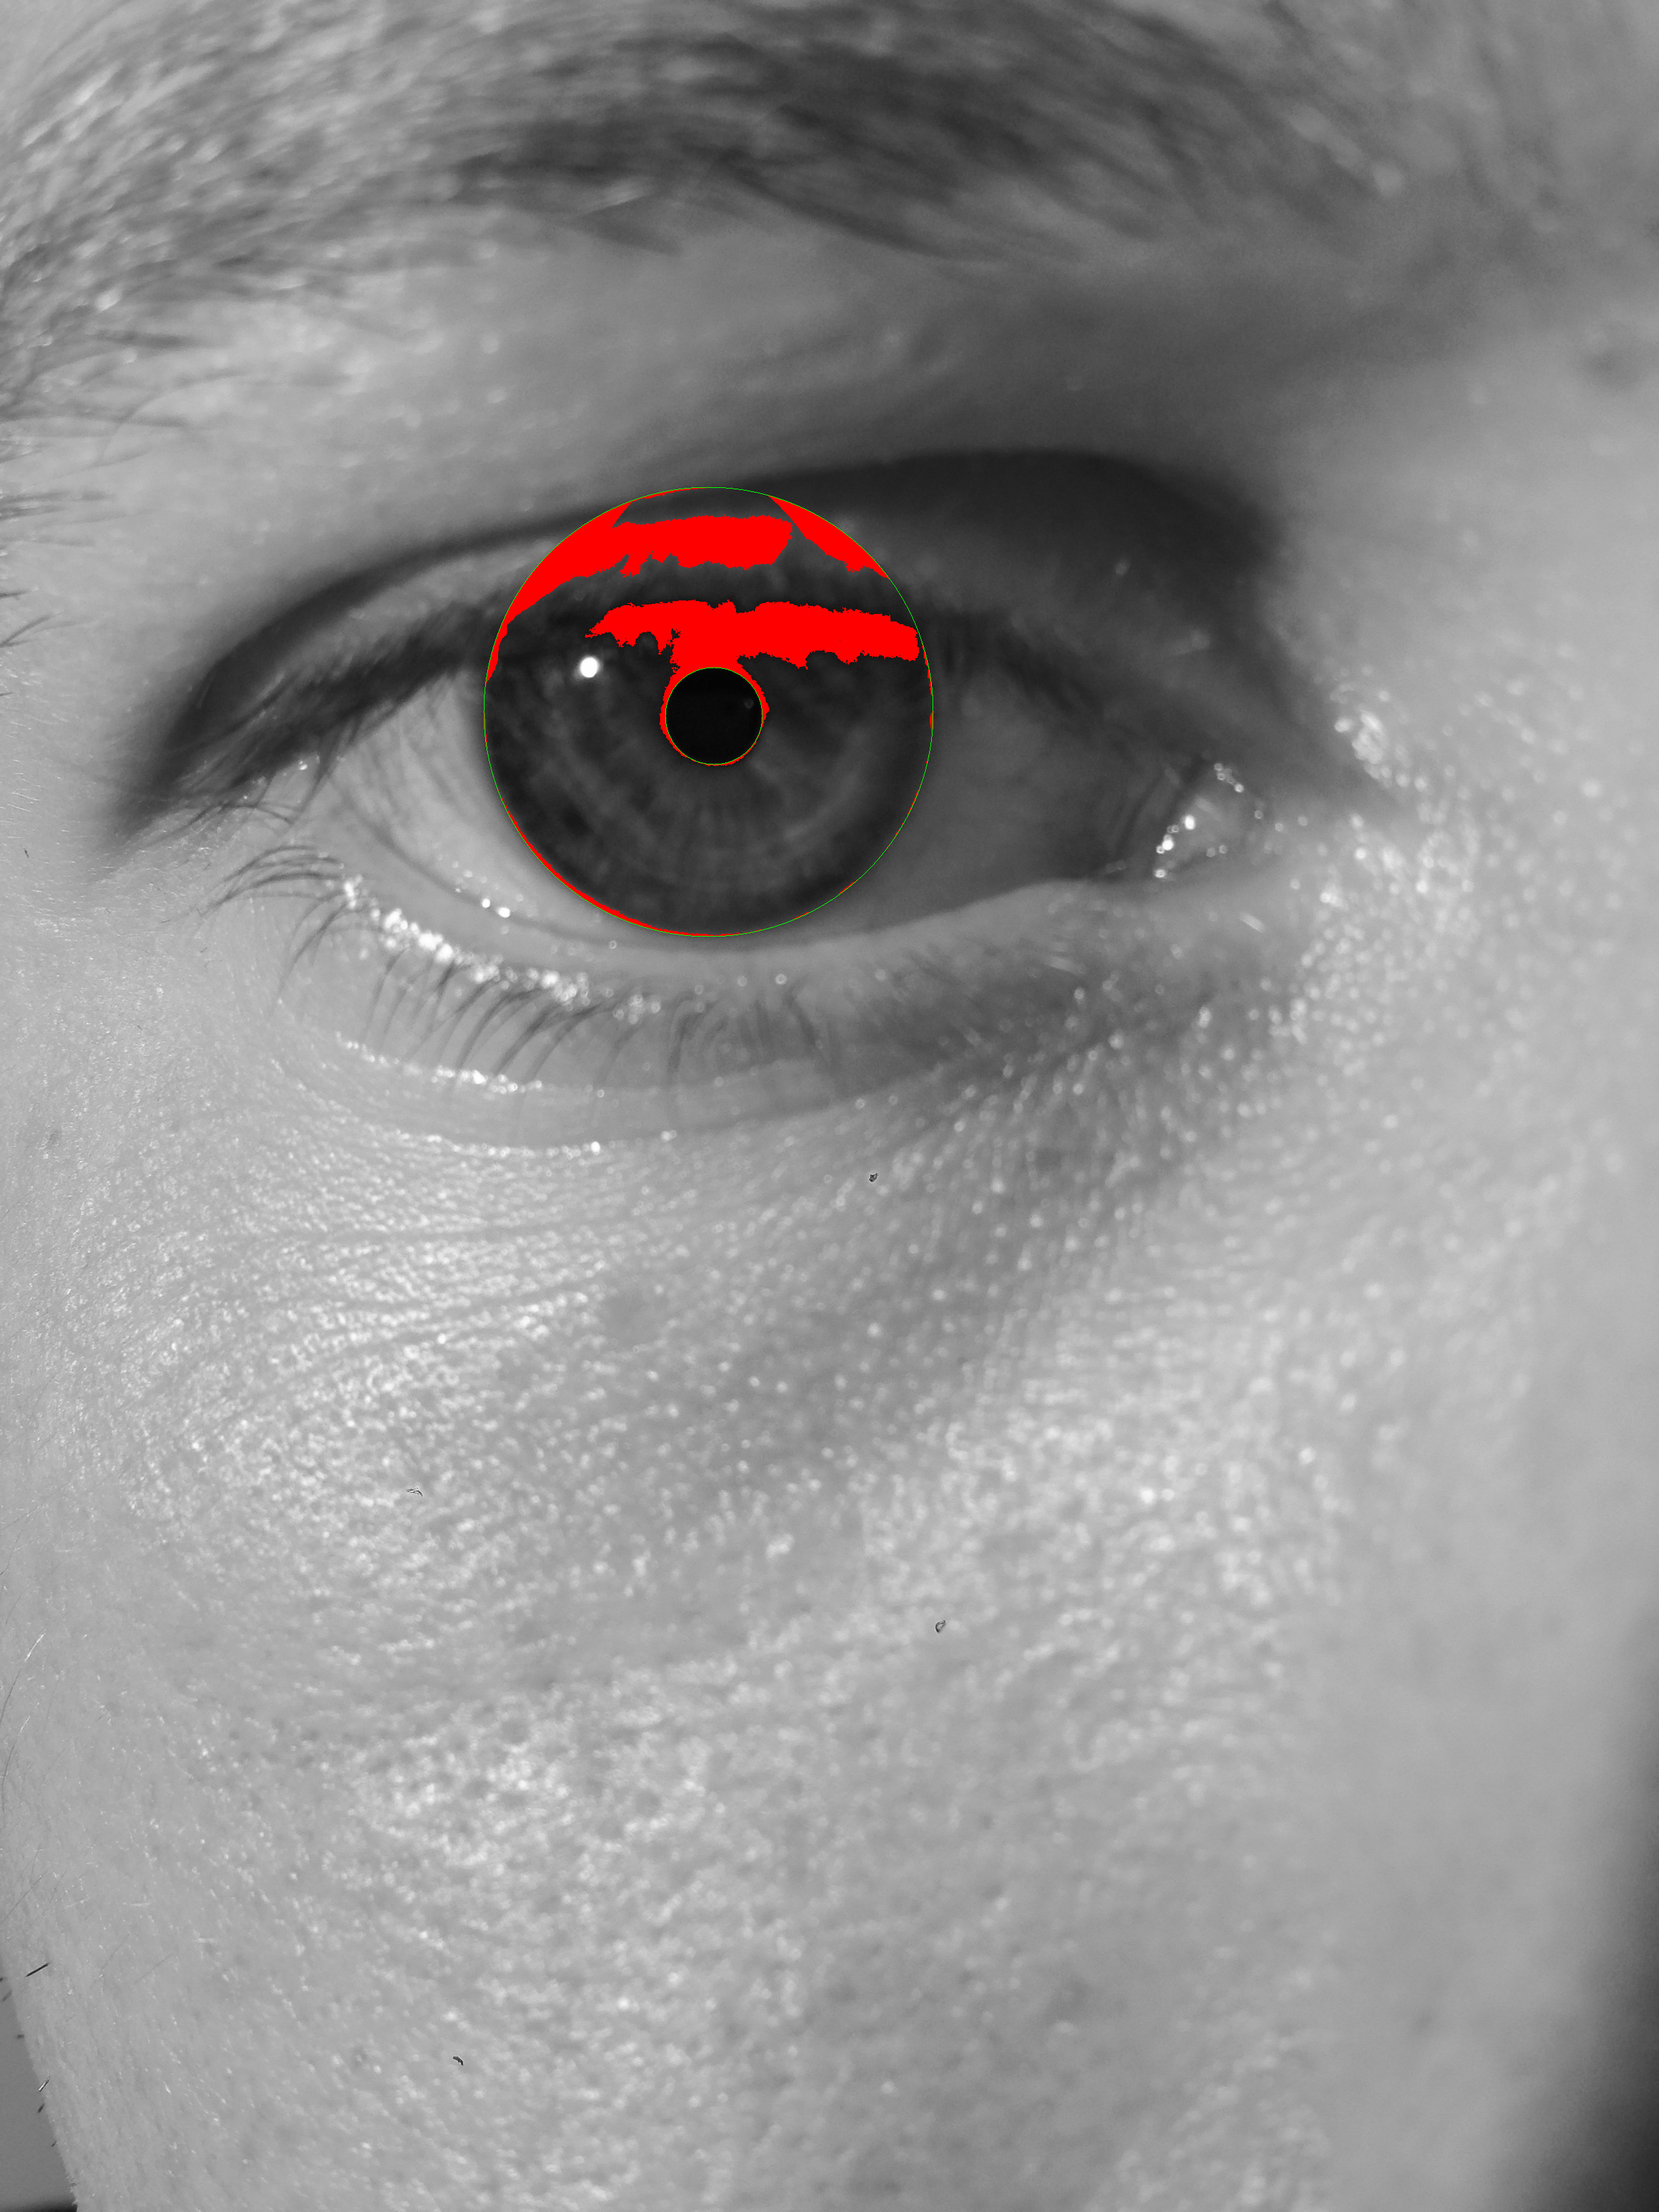
\includegraphics[width=\linewidth]{img/Resultados/miche/miche_seg_boa.jpg}
  \caption{Íris corretamente segmentada do \textit{MICHE}.}
\end{subfigure}\hfil % <-- added
\begin{subfigure}{0.25\textwidth}
  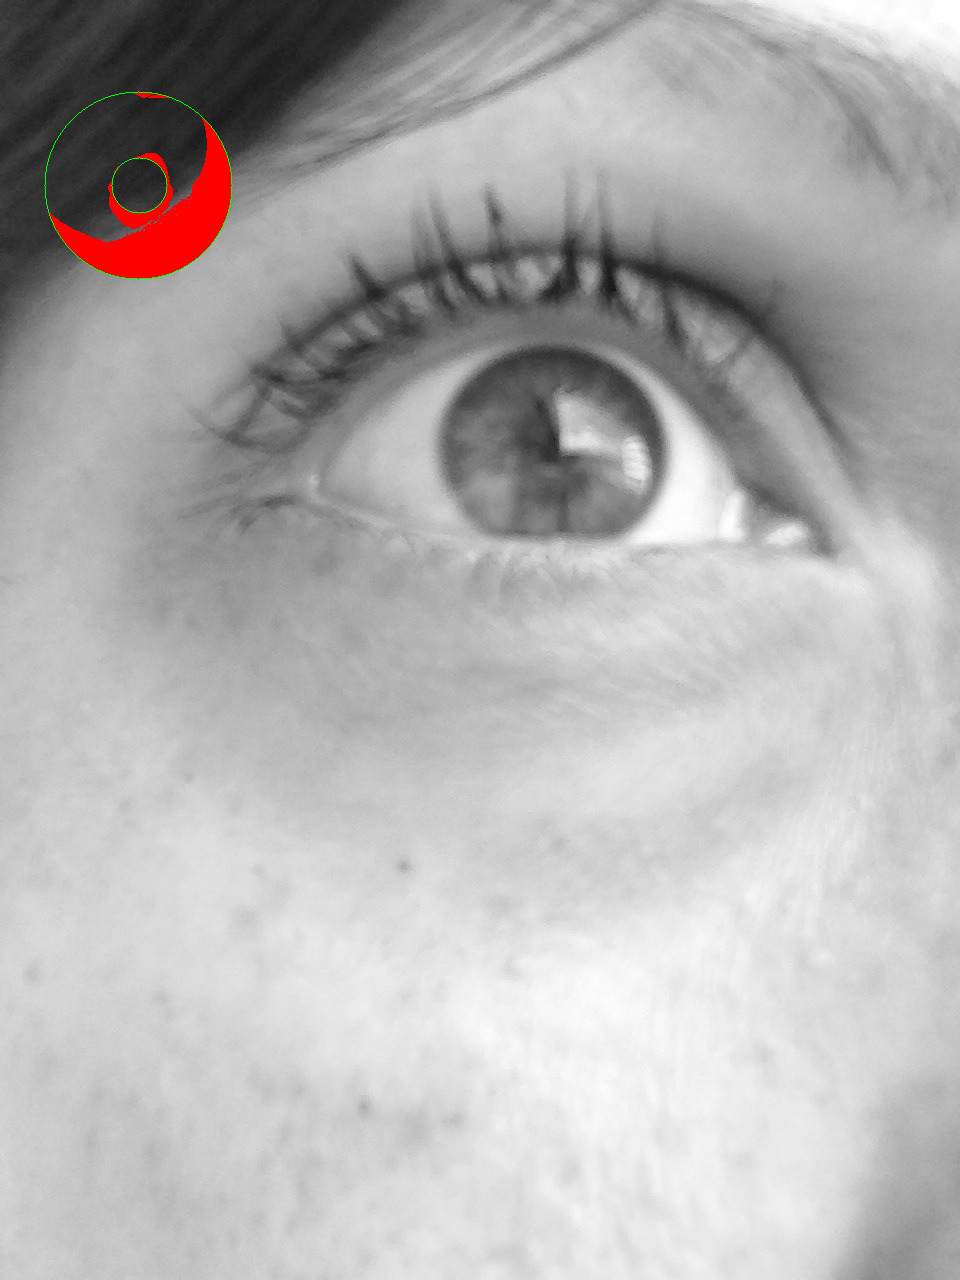
\includegraphics[width=\linewidth]{img/Resultados/miche/miche_seg_ruim.jpg}
  \caption{Íris incorretamente segmentada do \textit{MICHE}.}
\end{subfigure}\hfil % <-- added
\begin{subfigure}{0.25\textwidth}
  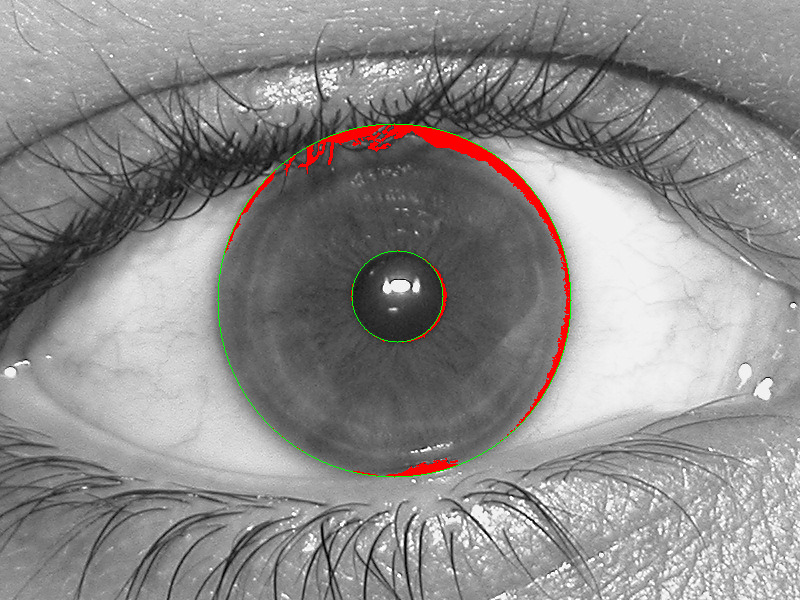
\includegraphics[width=\linewidth]{img/Resultados/ubirisv1/ubirisv1_seg_boa.jpg}
  \caption{Íris corretamente segmentada do \textit{UBIRISv1}.}
\end{subfigure}

\medskip
\begin{subfigure}{0.25\textwidth}
  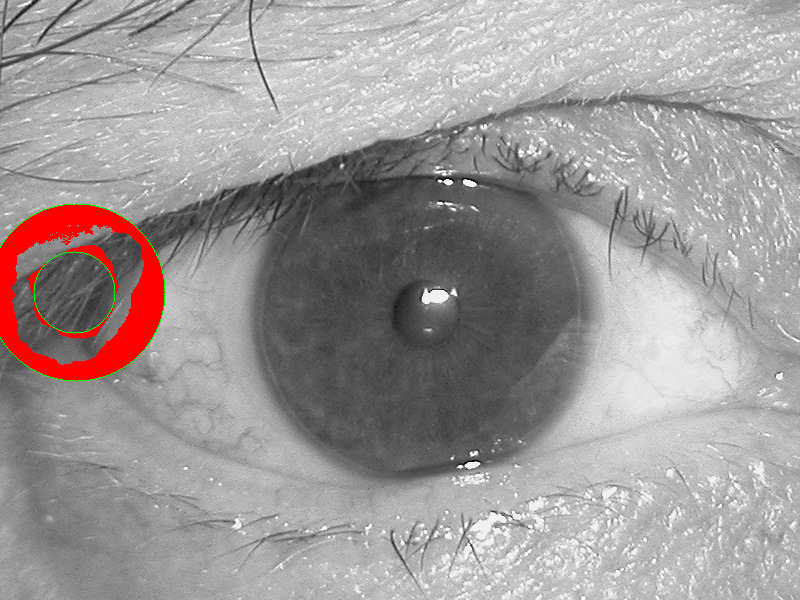
\includegraphics[width=\linewidth]{img/Resultados/ubirisv1/ubirisv1_seg_ruim.jpg}
  \caption{Íris incorretamente segmentada do \textit{UBIRISv1}.}
\end{subfigure}\hfil % <-- added
\begin{subfigure}{0.25\textwidth}
  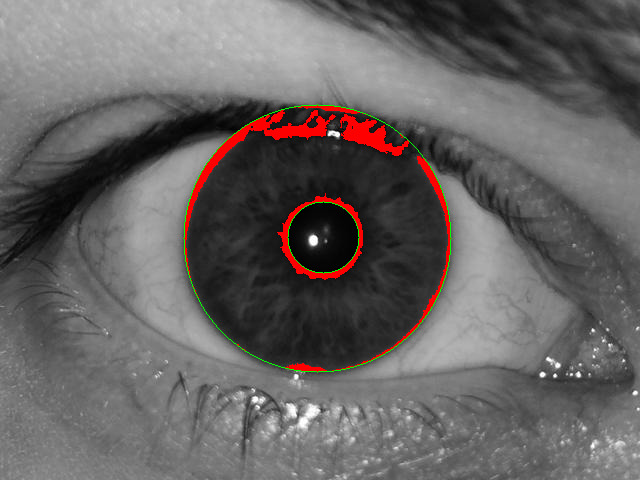
\includegraphics[width=\linewidth]{img/Resultados/warsaw/warsaw_seg_boa.jpg}
  \caption{Íris corretamente segmentada do \textit{\acrshort{Warsaw}}.}
\end{subfigure}\hfil % <-- added
\begin{subfigure}{0.25\textwidth}
  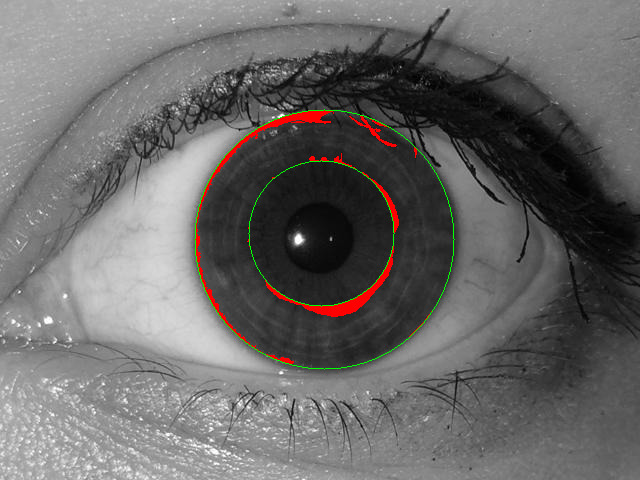
\includegraphics[width=\linewidth]{img/Resultados/warsaw/warsaw_seg_ruim.jpg}
  \caption{Íris incorretamente segmentada do \textit{\acrshort{Warsaw}}.}
\end{subfigure}
\caption{Resultados das segmentações de íris dos bancos de imagens \textit{MICHE, UBIRISv1} e \textit{\acrshort{Warsaw}}.}
\label{fig:experimentos:segmentacoes:todos}
\end{figure}

\begin{figure}[h!]
\begin{subfigure}{.25\textwidth}
\centering
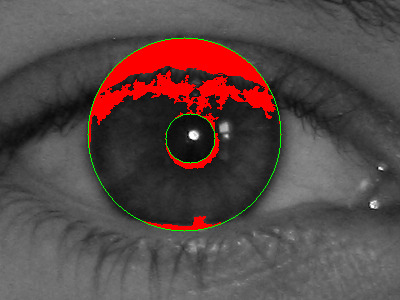
\includegraphics[width=\linewidth]{img/Resultados/ubirisv2/ubirisv2_seg_boa.jpg}
\caption{Íris corretamente segmentada.}
\end{subfigure}\hfill
\begin{subfigure}{.25\textwidth}
\centering
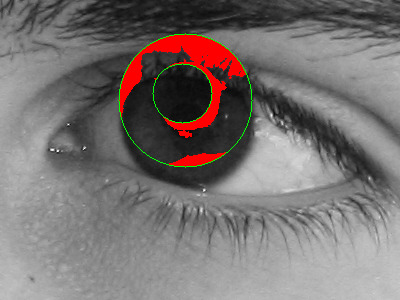
\includegraphics[width=\linewidth]{img/Resultados/ubirisv2/ubirisv2_seg_ruim1.jpg}
\caption{Imagem onde a segmentação da pupila apresentou erros.}
\end{subfigure}\hfill
\begin{subfigure}{.25\textwidth}
\centering
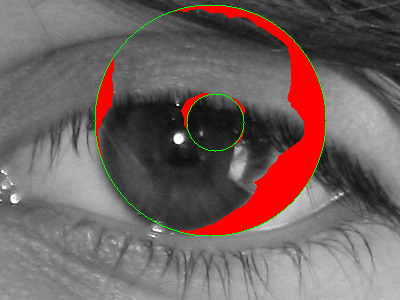
\includegraphics[width=\linewidth]{img/Resultados/ubirisv2/ubirisv2_seg_ruim2.jpg}
\caption{Imagem em que tanto a pupila quanto a íris foram incorretamente segmentadas.}
\end{subfigure}
\caption{Resultados da segmentação do banco de imagens \textit{UBIRISv2}.}
\label{fig:experimentos:segmentacoes:ubirisv2}
\end{figure}

\FloatBarrier

\section{Experimentos de Reconhecimento de Íris}\label{sec:experimentos:experimentos}

\par Cinco etapas foram seguidas para a realização dos experimentos em cada um dos bancos de imagens, e consistiram em:

\begin{enumerate}
    \item Executar a métrica \textit{\acrshort{DSMI}} em todas as imagens;
    \item Segmentar, normalizar e codificar todas as íris das imagens com o \textit{OSIRISv4.1};
    \item Executar a métrica \textit{\acrshort{FCE}} nos resultados da segmentação de todas as imagens;
    \item Executar o algoritmo de correspondência do \textit{OSIRISv4.1} com as \textit{IrisCodes} geradas para as íris;
    \item Aplicar os índices de rendimento de reconhecimento de íris nos resultados obtidos da correspondência das íris.
\end{enumerate}


\par A implementação da métrica de qualidade \textit{\acrshort{DSMI}} foi feita utilizando a linguagem de programação \textit{C++} com a biblioteca \textit{OpenCV} \cite{opencv}, assim como os códigos obtidos do sistema de reconhecimento de íris \textit{OSIRISv4.1}. A métrica de qualidade \textit{\acrshort{FCE}} e o cálculo dos índices de desempenho foram implementados na linguagem de programação \textit{Python} com o auxílio das bibliotecas \textit{Numpy} \cite{numpy}, \textit{scikit-learn} \cite{scikitlearn} e \textit{Matplotlib} \cite{matplotlib}.

% \begin{enumerate}
%     \item Gerar um arquivo texto com todas imagens (\textit{Todas\_Imagens});
%     \item Executar a métrica \textit{\acrshort{DSMI}} em todas as imagens no arquivo texto;
%     \item Aplicar o limiar $T_{DSMI}$ nas métricas \textit{\acrshort{DSMI}} calculadas e gerar um arquivo texto somente com as imagens com qualidade acima do limiar (\textit{Imagens\_DSMI});
%     \item Segmentar, normalizar e codificar todas as íris das imagens;
%     \item Executar a métrica \textit{\acrshort{FCE}} nos resultados da segmentação de todas as imagens;
%     \item Aplicar o limiar $T_{FCE}$ nas métricas \textit{\acrshort{FCE}} calculadas e gerar um arquivo texto somente com as imagens com qualidade acima do limiar (\textit{Imagens\_FCE});
%     \item Verificar as imagens que passaram nas duas métricas e gerar um arquivo texto com essas imagens (\textit{Imagens\_DSMI\_FCE});
%     \item Gerar os arquivos texto que comparam uma imagem com todas as outras a partir dos arquivos \textit{Todas\_Imagens}, \textit{Imagens\_DSMI}, \textit{Imagens\_FCE} e \textit{Imagens\_DSMI\_FCE};
%     \item Executar o algoritmo de correspondência do \textit{OSIRISv4.1} nos modelos gerados para as imagens dos arquivos texto da etapa 8;
%     \item Aplicar as métricas de rendimento de sistemas de reconhecimento de íris nos resultados do algoritmo de correspondência do \textit{OSIRISv4.1}.
% \end{enumerate}

\par Para analisar o rendimento da arquitetura de sistema de reconhecimento de íris proposta, foram utilizadas imagens originais e as ruidosas geradas para todos os bancos de imagens, como descrito na Seção \ref{sec:experimentos:ruidos}, totalizando 3000 por banco de imagens.

% \begin{itemize}
%     \item \acrfull{SR}: somente com as três imagens de teste de cada indivíduo dos bancos de imagens;
%     \item \acrfull{CR}: com as três imagens de teste e as geradas com ruídos (Seção \ref{sec:experimentos:ruidos}).
% \end{itemize}

% \par Para as duas categorias listadas acima, foram realizados quatro experimentos para avaliar o rendimento de sistemas de reconhecimento de íris de forma a comparar com o sistema proposto:

\par Foram realizados quatro experimentos com as imagens para avaliar o rendimento de sistemas de reconhecimento de íris de forma a comparar com o sistema proposto:

\begin{itemize}
    \item \acrfull{SM}: sistema padrão, sem usar métricas de qualidade;
    \item Usando somente a métrica de qualidade DSMI;
    \item Usando somente a métrica de qualidade FCE;
    \item \acrfull{DM}: Arquitetura proposta no projeto (\refFig{fig:metodologia:arquitetura}).
\end{itemize}

\par Para avaliar o desempenho dos quatro experimentos, os seguintes índices foram utilizadas:

\begin{itemize}
    \item \textit{\acrfull{AUC}} e \textit{\acrfull{ROC}} \cite{d33BEAT, aucROC, daugman2000};
    \item \textit{\acrfull{EER}} \cite{eer,d33BEAT};
    \item \textit{\acrfull{d'}} \cite{daugman2000}.
\end{itemize}

\subsection{\textit{\acrfull{AUC}} e \textit{\acrfull{ROC}}}\label{sec:experimentos:auc}

\par Sistemas biométricos devem aceitar ou rejeitar um indivíduo a partir de comparações de seus modelos com modelos armazenados \cite{wayman2005biometric}. A decisão de aceitar ou rejeitar um indivíduo pode resultar em quatro resultados: o indivíduo é corretamente aceito ou rejeitado ou é incorretamente aceito ou rejeitado. O limiar de decisão do sistema biométrico influencia diretamente nesses resultados. De forma a medir a acurácia de sistemas biométricos, quatro taxas são usadas \cite{daugman2000}:

\begin{enumerate}
    \item \textit{\acrfull{TPR}}: Taxa de indivíduos que são corretamente aceitos pelo sistema;
    \item \textit{\acrfull{TNR}}: Taxa de indivíduos que são corretamente rejeitados pelo sistema;
    \item \textit{\acrfull{FPR}}: Taxa de indivíduos que são incorretamente aceitos pelo sistema;
    \item \textit{\acrfull{FNR}}: Taxa de indivíduos que são incorretamente rejeitados pelo sistema.
\end{enumerate}

\par \textit{\acrshort{ROC}} é um gráfico comumente usado para avaliar o desempenho de sistemas de reconhecimento de íris \cite{aucROC, daugman2000}. O gráfico consiste na plotagem da \textit{\acrshort{TPR}} no eixo das ordenadas pela \textit{\acrshort{FPR}} no eixo das abcissas, que são calculadas para vários limiares de decisão. \textit{\acrshort{AUC}} é a métrica usada para avaliar o desempenho do sistema biométrico a partir do gráfico \textit{\acrshort{ROC}} e consiste em calcular a área sobre a curva do \textit{\acrshort{ROC}} \cite{aucROC}. A \textit{\acrshort{AUC}} qunatifica as aceitações e rejeições de indivíduos em sistemas biométricos. Pode resultar em valores entre 0.5 e 1, e possuem as seguintes classificações \cite{aucROC}:

\begin{itemize}
    \item Falha: 0.5 até 0.6;
    \item Pobre: 0.6 até 0.7;
    \item Justo: 0.7 até 0.8;
    \item Bom: 0.8 até 0.9;
    \item Excelente: 0.9 até 1.
\end{itemize}

A \refFig{fig:experimentos:roc_comruidos} ilustra os gráficos \textit{\acrshort{ROC}} e suas \textit{\acrshort{AUC}} calculadas para os experimentos.

\begin{figure}[H]
    \centering % <-- added
\begin{subfigure}{0.5\textwidth}
  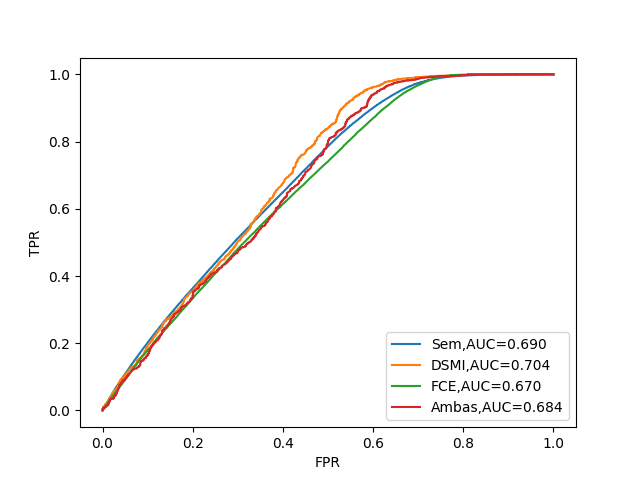
\includegraphics[width=\linewidth]{img/Resultados/miche_inter_distortion_auc.png}
  \caption{\textit{MICHE}.}
\end{subfigure}\hfil % <-- added
\begin{subfigure}{0.5\textwidth}
  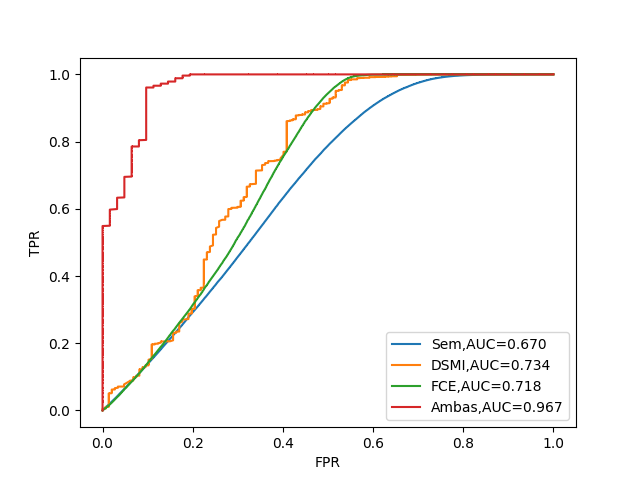
\includegraphics[width=\linewidth]{img/Resultados/ubirisv1_inter_distortion_auc.png}
  \caption{\textit{UBIRISv1}.}
\end{subfigure}

\medskip
\begin{subfigure}{0.5\textwidth}
  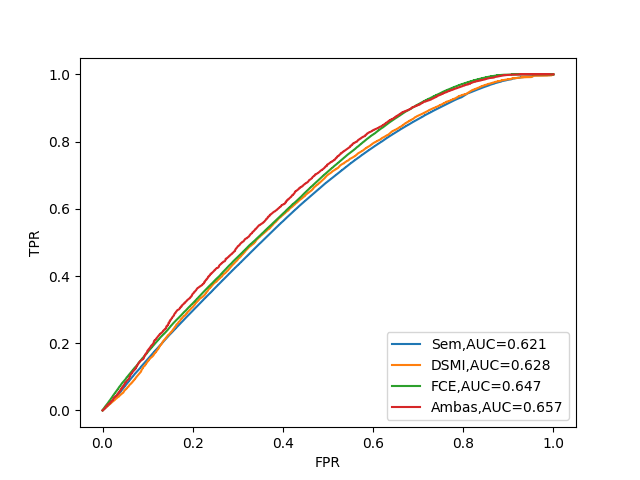
\includegraphics[width=\linewidth]{img/Resultados/ubirisv2_inter_distortion_auc.png}
  \caption{\textit{UBIRISv2}.}
\end{subfigure}\hfil % <-- added
\begin{subfigure}{0.5\textwidth}
  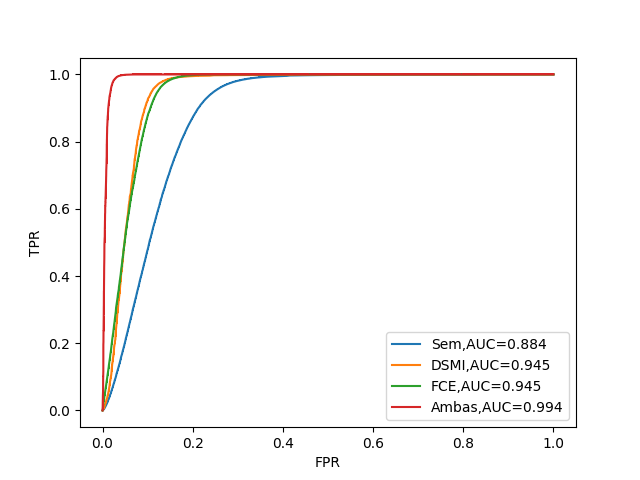
\includegraphics[width=\linewidth]{img/Resultados/warsaw_inter_distortion_auc.png}
  \caption{{\acrshort{Warsaw}}.}
\end{subfigure}\hfil % <-- added
\caption{Curvas \textit{\acrshort{ROC}} e \textit{\acrshort{AUC}} calculados para as imagens do experimento de cada banco de imagens. Nos gráficos, \textit{Sem} são as \textit{\acrshort{AUC}} que foram calculadas sem nenhuma métrica de qualidade e \textit{Ambas} significa \textit{\acrshort{AUC}} calculadas com as duas métricas de qualidade.}
\label{fig:experimentos:roc_comruidos}
\end{figure}

\par No banco de imagens \textit{MICHE}, a arquitetura proposta com as duas métricas de qualidade não apresentou o melhor resultado no experimento. Usando somente a métrica \textit{\acrshort{DSMI}} apresentou a melhor \textit{\acrshort{AUC}}, mas o seu valor calculado, no entanto, é considerado somente justo \cite{aucROC}, com valor no intervalo 0.7 a 0.8.

\par No banco de imagens \textit{\acrshort{Warsaw}}, a arquitetura proposta com as duas métricas obteve a melhor \textit{\acrshort{AUC}}. O resultado encontrado com a arquitetura proposta no experimento é excelente \cite{aucROC}, porque apresenta \textit{\acrshort{AUC}} no intervalos 0.9 a 1.

\par Nos bancos de imagens \textit{UBIRISv1} e \textit{UBIRISv2}, a arquitetura proposta obteve os melhores resultados no experimento. A \textit{\acrshort{AUC}} calculada no \textit{UBIRISv1} foi excelente e apresentou valor entre 0.9 e 1 \cite{aucROC}. Apesar da arquitetura proposta ter apresentado o melhor resultado no experimento do \textit{UBIRISv2}, a \textit{\acrshort{AUC}} calculada foi pobre \cite{aucROC}, apresentando valores entre 0.6 e 0.7.

\par Portanto, pelas \textit{\acrshort{AUC}} calculados, pode-se afirmar que com pelo menos uma métrica de qualidade, o desempenho de sistemas de reconhecimento de íris é melhorado, onde em um banco de imagens usando somente a métrica de qualidade \textit{\acrshort{DSMI}} obteve o melhor resultado e nos outros três bancos de imagens a arquitetura proposta obteve os melhores resultados. 

\FloatBarrier

\subsection{\textit{\acrfull{EER}}} \label{sec:experimentos:eer}

\par \textit{\acrshort{EER}} é uma métrica utilizada para calcular o desempenho de sistemas biométricos \cite{eer}. É calculada, assim como \textit{\acrshort{AUC}}, com base nas taxas \textit{\acrshort{TPR}}, \textit{\acrshort{TNR}}, \textit{\acrshort{FPR}} e \textit{\acrshort{FNR}} resultantes do processo de decisão do sistema. A taxa \textit{\acrshort{EER}} consiste no ponto em que as taxas de erro \textit{\acrshort{FPR}} e \textit{\acrshort{FNR}} são iguais, conforme as Equações \ref{eq:experimentos:eer} e \ref{eq:experimentos:eer_T} \cite{d33BEAT}:

\equacao{eq:experimentos:eer}{
    EER = FPR(T_{*}) = FNR(T_{*}),
}

\noindent onde 

\equacao{eq:experimentos:eer_T}{
    T_{*} = arg \underset{T}{min}(|FPR(T) - FNR(T)|)
}

\noindent é o limiar de decisão que melhor aproxima a igualdade da \refEq{eq:experimentos:eer}. Quanto mais próximo de 0 for a \textit{\acrshort{EER}} calculada, melhor o desempenho do sistema \cite{d33BEAT}. Na \refTab{tab:experimentos:eer}, os \textit{\acrshort{EER}} calculados para todos os experimentos são apresentados.
% e na \refTab{tab:experimentos:limiar_eer} os limiares $T_{FCE}$ da \refEq{eq:experimentos:eer_T}.

\begin{table}[h!]
\centering
\caption{Valores calculados para \textit{\acrshort{EER}} dos bancos de imagens.}
\label{tab:experimentos:eer}
\begin{tabular}{l|l|l|l|l|}
\cline{2-5}
 & \textit{\textbf{MICHE}} & \textit{\textbf{UBIRISv1}} & \textit{\textbf{UBIRISv2}} & \textit{\textbf{Warsaw}} \\ \hline
\multicolumn{1}{|l|}{\textbf{SM}} & 0.379 & 0.388 & 0.416 & 0.180 \\ \hline
\multicolumn{1}{|l|}{\textbf{DSMI}} & \textbf{0.370} & 0.327 & 0.408 & 0.095 \\ \hline
\multicolumn{1}{|l|}{\textbf{FCE}} & 0.394 & 0.355 & 0.407 & 0.105 \\ \hline
\multicolumn{1}{|l|}{\textbf{DM}} & 0.392 & \textbf{0.097} & \textbf{0.394} & \textbf{0.023} \\ \hline
\end{tabular}
\end{table}

% \begin{table}[h!]
% \centering
% \caption{Valores calculados para \textit{\acrshort{EER}} dos bancos de imagens.}
% \label{tab:experimentos:eer}
% \tabcolsep=0.09cm
% \begin{tabular}{l|l|l|l|l|l|l|l|l|}
% \cline{2-9}
%  & \multicolumn{2}{c|}{\textit{\textbf{MICHE}}} & \multicolumn{2}{c|}{\textit{\textbf{UBIRISv1}}} & \multicolumn{2}{c|}{\textit{\textbf{UBIRISv2}}} & \multicolumn{2}{c|}{\textit{\textbf{Warsaw}}} \\ \cline{2-9} 
%  & \multicolumn{1}{c|}{\textbf{SR}} & \multicolumn{1}{c|}{\textbf{CR}} & \multicolumn{1}{c|}{\textbf{SR}} & \multicolumn{1}{c|}{\textbf{CR}} & \multicolumn{1}{c|}{\textbf{SR}} & \multicolumn{1}{c|}{\textbf{CR}} & \multicolumn{1}{c|}{\textbf{SR}} & \multicolumn{1}{c|}{\textbf{CR}} \\ \hline
% \multicolumn{1}{|l|}{\textbf{SM}} & 0.367 & 0.379 & 0.357 & 0.388 & 0.428 & 0.416 & 0.058 & 0.180 \\ \hline
% \multicolumn{1}{|l|}{\textbf{DSMI}} & 0.388 & \textbf{0.370} & 0.327 & 0.327 & 0.435 & 0.408 & 0.063 & 0.095 \\ \hline
% \multicolumn{1}{|l|}{\textbf{FCE}} & \textbf{0.333} & 0.394 & 0.247 & 0.355 & 0.386 & 0.407 & \textbf{0.018} & 0.105 \\ \hline
% \multicolumn{1}{|l|}{\textbf{DM}} & 0.341 & 0.392 & \textbf{0.097} & \textbf{0.097} & \textbf{0.381} & \textbf{0.394} & 0.028 & \textbf{0.023} \\ \hline
% \end{tabular}
% \end{table}

\par A melhor \textit{\acrshort{EER}} calculada para o banco de imagens \textit{MICHE} foi usando somente a métrica de qualidade \textit{\acrshort{DSMI}}. O valor calculado, assim como aquele encontrado para \textit{\acrshort{AUC}}, são valores regulares, porque quanto maior a \textit{\acrshort{EER}}, pior o desempenho do sistema \cite{eer, d33BEAT} e reafirmam a dificuldade do \textit{MICHE}.

% \par As melhores \textit{\acrshort{EER}} calculadas para o banco de imagens \textit{MICHE} foram usando somente as métrica \textit{\acrshort{FCE}} e \textit{\acrshort{DSMI}} nos experimentos sem ruído e com ruído, respectivamente. Esses valores, assim como os encontrados para \textit{\acrshort{AUC}}, são valores ruins, porque quanto maior a \textit{\acrshort{EER}}, pior o desempenho do sistema \cite{eer, d33BEAT} e reafirmam a dificuldade do  \textit{MICHE}.

\par Assim como no experimento da \textit{\acrshort{AUC}}, a melhor \textit{\acrshort{EER}} do banco de imagens \textit{\acrshort{Warsaw}} foi calculada usando a arquitetura proposta. Os valores também são excelentes, porque são próximos de 0 \cite{eer, d33BEAT}.

% \par Assim como nos testes da \textit{\acrshort{AUC}}, as melhores \textit{\acrshort{EER}} do banco de imagens \textit{\acrshort{Warsaw}} sem e com ruídos foram calculadas usando somente a métrica \textit{\acrshort{FCE}} e na arquitetura proposta. Os avalores também são excelentes, porque são próximos de 0 \cite{eer, d33BEAT}.

\par A arquitetura proposta, assim como na métrica \textit{\acrshort{AUC}}, apresentou os melhores resultados nos bancos de imagens \textit{UBIRISv1} e \textit{UBIRISv2}. E assim como os resultados de \textit{\acrshort{AUC}}, o valor apresentado no \textit{UBIRISv2} é considerado fraco, porque é uma \textit{\acrshort{EER}} elevada e no \textit{UBIRISv1} é excelente, com valor perto de 0 \cite{eer, d33BEAT}.

\par A arquitetura proposta obteve os melhores resultados em três dos quatro bancos de imagens e usando a métrica de qualidade \textit{\acrshort{DSMI}} no outro. Pode-se afirmar pelos resultados das \textit{\acrshort{EER}}, portanto, que métricas de qualidade influenciam no desempenho de sistemas de reconhecimento de íris.

% \begin{table}[h!]
% \centering
% \caption{Limiares de decisão encontrados a partir do \textit{\acrshort{EER}} ($T_{FCE}$).}
% \label{tab:experimentos:limiar_eer}
% \tabcolsep=0.09cm
% \begin{tabular}{l|l|l|l|l|l|l|l|l|}
% \cline{2-9}
%  & \multicolumn{2}{c|}{\textit{\textbf{MICHE}}} & \multicolumn{2}{c|}{\textit{\textbf{UBIRISv1}}} & \multicolumn{2}{c|}{\textit{\textbf{UBIRISv2}}} & \multicolumn{2}{c|}{\textit{\textbf{Warsaw}}} \\ \cline{2-9} 
%  & \multicolumn{1}{c|}{\textbf{SR}} & \multicolumn{1}{c|}{\textbf{CR}} & \multicolumn{1}{c|}{\textbf{SR}} & \multicolumn{1}{c|}{\textbf{CR}} & \multicolumn{1}{c|}{\textbf{SR}} & \multicolumn{1}{c|}{\textbf{CR}} & \multicolumn{1}{c|}{\textbf{SR}} & \multicolumn{1}{c|}{\textbf{CR}} \\ \hline
% \multicolumn{1}{|l|}{\textbf{SM}} & 0.424020 & 0.431624 & 0.431900 & 0.433628 & 0.426407 & 0.429078 & 0.408257 & 0.428270 \\ \hline
% \multicolumn{1}{|l|}{\textbf{DSMI}} & 0.425373 & 0.431090 & 0.428070 & 0.428070 & 0.429293 & 0.430233 & 0.410030 & 0.419355 \\ \hline
% \multicolumn{1}{|l|}{\textbf{FCE}} & 0.426117 & 0.441176 & 0.425926 & 0.437984 & 0.423810 & 0.441667 & 0.404762 & 0.427305 \\ \hline
% \multicolumn{1}{|l|}{\textbf{DM}} & 0.430556 & 0.439655 & 0.406250 & 0.406250 & 0.427083 & 0.438172 & 0.407986 & 0.40833 \\ \hline
% \end{tabular}
% \end{table}

\FloatBarrier

\subsection{\textit{\acrfull{d'}}}\label{sec:experimentos:daugman}

\par O limiar de decisão do sistema biométrico que influencia nas taxa de acerto e erro nas correspondências. Quanto mais conservador, maior a \textit{\acrshort{FNR}} e quanto menos criterioso, maior a \textit{\acrshort{FPR}} \cite{daugman2000}. As sobreposições das distribuições das \acrlong{HD} de correspondências aceitas e rejeitadas quantificam o poder de decisão do sistema, e essas sobreposições consistem nas taxas \textit{\acrshort{FPR}} e \textit{\acrshort{FNR}}. A métrica \textit{\acrshort{d'}} foi proposta de forma a calcular a separação da distribuição das íris aceitas e rejeitadas, o grau de detrimento entre as duas taxas de erro e quantificar em um valor a capacidade de decisão de um sistema de reconhecimento de íris, e é descrita pela \refEq{eq:experimentos:daugman} \cite{daugman2000}:

\equacao{eq:experimentos:daugman}{
    d' = \frac{|\mu_{1} - \mu_{2}|}{\sqrt{\frac{1}{2}(\sigma_{1}^2 + \sigma_{2}^2)}},
}

\noindent onde $\mu_{1}$ e $\mu_{2}$ são as médias das \textit{\acrlong{HD}} das íris que foram aceitas e rejeitadas, respectivamente, enquanto $\sigma_{1}^2$ e $\sigma_{2}^2$ são seus desvios padrões. Quanto maior o valor de \textit{\acrshort{d'}}, melhor o poder de decisão do sistema de reconhecimento de íris.

\par Nos experimentos realizados, \textit{\acrshort{d'}} foi calculado utilizando quatro limiares de decisão: $T_{1} = 0.2$, $T_{2} = 0.3$, $T_{3} = 0.4$ e $T_{EER}$. $T_{EER}$ consiste nos limiares encontrados no ponto da \textit{\acrshort{EER}}.
% , e são enumerados na \refTab{tab:experimentos:limiar_eer}.

% \begin{table}[h!]
% \centering
% \caption{Limiares utilizados para o cálculo do \textit{\acrshort{d'}}}
% \label{tab:experimentos:limiares}
% \begin{tabular}{l|l|l|l|}
% \cline{2-4}
%  & $T_{1}$ & $T_{2}$ & $T_{3}$ \\ \hline
% \multicolumn{1}{|l|}{\textbf{Limiar}} & 0.2 & 0.3 & 0.4 \\ \hline
% \end{tabular}
% \end{table}


% \begin{table}[h!]
% \centering
% \caption{Valores calculados para \textit{\acrshort{d'}} nas imagens sem ruídos.}
% \label{tab:experimentos:d:sem_ruido}
% \tabcolsep=0.02cm
% \begin{tabular}{l|l|l|l|l|l|l|l|l|l|l|l|l|l|l|l|l|}
% \cline{2-17}
%  & \multicolumn{4}{c|}{\textit{\textbf{MICHE}}} & \multicolumn{4}{c|}{\textit{\textbf{UBIRISv1}}} & \multicolumn{4}{c|}{\textit{\textbf{UBIRISv2}}} & \multicolumn{4}{c|}{\textit{\textbf{Warsaw}}} \\
%  \cline{2-17} &
% \multicolumn{1}{c|} {\textbf{$T_{1}$}} & \textbf{$T_{2}$} & \textbf{$T_{3}$} & \textbf{$T_{EER}$} & \textbf{$T_{1}$} & \textbf{$T_{2}$} & \textbf{$T_{3}$} & \textbf{$T_{EER}$} & \textbf{$T_{1}$} & \textbf{$T_{2}$} & \textbf{$T_{3}$} & \textbf{$T_{EER}$} & \textbf{$T_{1}$} & \textbf{$T_{2}$} & \textbf{$T_{3}$} & \textbf{$T_{EER}$} \\ \hline
% \multicolumn{1}{|l|}{\textbf{SM}} & 5.78 & 3.40 & \textbf{2.35} & \textbf{2.23} & 7.19 & 3.26 & \textbf{2.26} & 1.85 & 4.43 & 2.73 & 1.81 & 1.67 & 10.49 & 7.04 & 1.84 & 1.66 \\ \hline
% \multicolumn{1}{|l|}{\textbf{DSMI}} & 5.75 & 3.56 & 2.19 & 2.10 & 6.74 & 4.16 & 2.21 & \textbf{1.86} & 4.37 & 2.65 & 1.71 & 1.56 & 10.46 & 6.66 & 1.89 & 1.62 \\ \hline
% \multicolumn{1}{|l|}{\textbf{FCE}} & 6.87 & 3.97 & 1.99 & 2.01 & \textbf{9.96} & 6.06 & 1.66 & 1.29 & \textbf{16.48} & 5.65 & 2.73 & \textbf{2.65} & \textbf{11.44} & \textbf{8.83} & \textbf{2.44} & \textbf{2.03} \\ \hline
% \multicolumn{1}{|l|}{\textbf{DM}} & \textbf{7.68} & \textbf{4.22} & 1.70 & 1.68 & 9.42 & \textbf{6.49} & 1.74 & 1.55 & 16.26 & \textbf{6.48} & \textbf{2.84} & 2.63 & 11.04 & 8.09 & 2.29 & 1.79 \\ \hline
% \end{tabular}
% \end{table}

%Isso pode ser explicado porque quanto menor os limiares, mais criterioso é o sistema, e menos correspondência são aceitas, de forma que a diferença absoluta de suas médias é maior

\begin{table}[h!]
\centering
\caption{Valores calculados para \textit{\acrshort{d'}} nos experimentos.}
\label{tab:experimentos:d:com_ruido}
\resizebox{1\textwidth}{!}{%
\begin{tabular}{l|l|l|l|l|l|l|l|l|l|l|l|l|l|l|l|l|}
\cline{2-17}
 & \multicolumn{4}{c|}{\textit{\textbf{MICHE}}} & \multicolumn{4}{c|}{\textit{\textbf{UBIRISv1}}} & \multicolumn{4}{c|}{\textit{\textbf{UBIRISv2}}} & \multicolumn{4}{c|}{\textit{\textbf{Warsaw}}} \\
 \cline{2-17} &
\multicolumn{1}{c|} {\textbf{$T_{1}$}} & \textbf{$T_{2}$} & \textbf{$T_{3}$} & \textbf{$T_{EER}$} & \textbf{$T_{1}$} & \textbf{$T_{2}$} & \textbf{$T_{3}$} & \textbf{$T_{EER}$} & \textbf{$T_{1}$} & \textbf{$T_{2}$} & \textbf{$T_{3}$} & \textbf{$T_{EER}$} & \textbf{$T_{1}$} & \textbf{$T_{2}$} & \textbf{$T_{3}$} & \textbf{$T_{EER}$} \\ \hline
\multicolumn{1}{|l|}{\textbf{SM}} & 5.70 & 3.48 & 2.13 & 1.94 & 6.57 & 3.86 & \textbf{2.29} & \textbf{1.92} & 3.99 & 2.67 & 1.68 & 1.48 & 7.38 & 4.70 & 1.88 & 1.42 \\ \hline
\multicolumn{1}{|l|}{\textbf{DSMI}} & 6.10 & 3.86 & 2.34 & 2.17 & 6.74 & 4.16 & 2.21 & 1.86 & 4.09 & 2.67 & 1.62 & 1.41 & 7.62 & 4.82 & 2.06 & 1.56 \\ \hline
\multicolumn{1}{|l|}{\textbf{FCE}} & \textbf{7.24} & \textbf{4.13} & 1.91 & 1.82 & 8.33 & 5.06 & 1.72 & 1.45 & \textbf{8.10} & \textbf{3.96} & 2.39 & 2.26 & \textbf{8.43} & \textbf{5.16} & 2.26 & 1.31 \\ \hline
\multicolumn{1}{|l|}{\textbf{DM}} & 6.51 & 4.10 & \textbf{2.37} & \textbf{2.18} & \textbf{9.42} & \textbf{6.49} & 1.74 & 1.55 & 7.29 & 3.86 & \textbf{2.61} & \textbf{2.42} & 7.82 & 5.04 & \textbf{2.44} & \textbf{1.95} \\ \hline
\end{tabular}
}

\end{table}

% \begin{table}[h!]
% \centering
% \caption{Valores calculados para \textit{\acrshort{d'}} nos experimentos.}
% \label{tab:experimentos:d:com_ruido}
% \tabcolsep=0.04cm
% \begin{tabular}{l|l|l|l|l|l|l|l|l|l|l|l|l|l|l|l|l|}
% \cline{2-17}
%  & \multicolumn{4}{c|}{\textit{\textbf{MICHE}}} & \multicolumn{4}{c|}{\textit{\textbf{UBIRISv1}}} & \multicolumn{4}{c|}{\textit{\textbf{UBIRISv2}}} & \multicolumn{4}{c|}{\textit{\textbf{Warsaw}}} \\
%  \cline{2-17} &
% \multicolumn{1}{c|} {\textbf{$T_{1}$}} & \textbf{$T_{2}$} & \textbf{$T_{3}$} & \textbf{$T_{EER}$} & \textbf{$T_{1}$} & \textbf{$T_{2}$} & \textbf{$T_{3}$} & \textbf{$T_{EER}$} & \textbf{$T_{1}$} & \textbf{$T_{2}$} & \textbf{$T_{3}$} & \textbf{$T_{EER}$} & \textbf{$T_{1}$} & \textbf{$T_{2}$} & \textbf{$T_{3}$} & \textbf{$T_{EER}$} \\ \hline
% \multicolumn{1}{|l|}{\textbf{SM}} & 5.70 & 3.48 & 2.13 & 1.94 & 6.57 & 3.86 & \textbf{2.29} & \textbf{1.92} & 3.99 & 2.67 & 1.68 & 1.48 & 7.38 & 4.70 & 1.88 & 1.42 \\ \hline
% \multicolumn{1}{|l|}{\textbf{DSMI}} & 6.10 & 3.86 & 2.34 & 2.17 & 6.74 & 4.16 & 2.21 & 1.86 & 4.09 & 2.67 & 1.62 & 1.41 & 7.62 & 4.82 & 2.06 & 1.56 \\ \hline
% \multicolumn{1}{|l|}{\textbf{FCE}} & \textbf{7.24} & \textbf{4.13} & 1.91 & 1.82 & 8.33 & 5.06 & 1.72 & 1.45 & \textbf{8.10} & \textbf{3.96} & 2.39 & 2.26 & \textbf{8.43} & \textbf{5.16} & 2.26 & 1.31 \\ \hline
% \multicolumn{1}{|l|}{\textbf{DM}} & 6.51 & 4.10 & \textbf{2.37} & \textbf{2.18} & \textbf{9.42} & \textbf{6.49} & 1.74 & 1.55 & 7.29 & 3.86 & \textbf{2.61} & \textbf{2.42} & 7.82 & 5.04 & \textbf{2.44} & \textbf{1.95} \\ \hline
% \end{tabular}
% \end{table}

% \par Tanto nos experimentos sem ruído quanto com ruído, os valores do \textit{\acrshort{d'}} calculados apresentaram os melhores resultados com os menores limiares. Isso pode ser explicado porque quanto menor o limiar, menor a média dos valores da \textit{\acrshort{HD}} das comparações aceitas, e como a média das \textit{\acrshort{HD}} das comparações rejeitadas mantém-se praticamente constante, o numerador da \refEq{eq:experimentos:daugman} aumenta e os seus resultados consequentemente. As Tabelas \ref{tab:experimentos:media_sem_ruidos_daugman} e \ref{tab:experimentos:media_com_ruidos_daugman} no \refApendice{Apendice_B} enumeram as médias, variâncias e quantidade de comparações aceitas e rejeitadas calculadas para os experimentos sem ruído.

\par Nos experimentos, os valores do \textit{\acrshort{d'}} calculados apresentaram os melhores resultados com os menores limiares. Isso pode ser explicado porque quanto menor o limiar, menor a média dos valores da \textit{\acrshort{HD}} das comparações aceitas, e como a média das \textit{\acrshort{HD}} das comparações rejeitadas mantém-se praticamente constante, o numerador da \refEq{eq:experimentos:daugman} aumenta e os seus resultados consequentemente. 

% \par Nos experimentos sem ruído, a arquitetura proposta com as duas métricas de qualidade apresentaram os melhores resultados do índice \textit{\acrshort{d'}} com os limiares $T_{1}$ e $T_{2}$ no banco de imagens \textit{MICHE}. O banco de imagens \textit{UBIRISv1} apresentou o melhor valor de \textit{\acrshort{d'}} com a arquitetura proposta somente com o limiar $T_{2}$. No banco de imagens \textit{UBIRISv2}, a arquitetura proposta obteve os maiores valores no experimento com os limiares $T_{2}$ e $T_{3}$. Por fim, no banco de imagens \textit{\acrshort{Warsaw}}, a arquitetura proposta, contrariando os bons resultados obtidos com as métricas \textit{\acrshort{AUC}} e \textit{\acrshort{EER}}, não obteve o melhor resultado com nenhum dos limiares.

\par O banco de imagens \textit{MICHE} apresentou os maiores índices com a arquitetura proposta com os limiares $T_{3}$ e $T_{EER}$. No \textit{UBIRISv1}, os dois maiores valores com a arquitetura proposta foram calculados com dois limiares: $T_{1}$ e $T_{2}$. O banco de imagens \textit{UBIRISv2} também apresentou dois maiores valores com a arquitetura proposta com os limiares $T_{2}$ e $T_{3}$. Os resultados encontrados com a arquitetura proposta no \textit{\acrshort{Warsaw}} apresentou os maiores valores em dois limiares no índice: $T_{3}$ e $T_{EER}$. O único banco de imagens que apresentou valores maiores sem nenhuma métrica de qualidade, foi o \textit{UBIRISv1}, com os limiares $T_{3}$ e $T_{EER}$, e pode ser explicado porque apesar da diferença absoluta das médias ter sido pequena, as suas variâncias calculadas foram menores que as usando métricas de qualidade, de forma que os valores do \textit{\acrshort{d'}} foram maiores.

% \par Já nos experimentos com ruídos, o banco de imagens \textit{MICHE} apresentou os maiores índices com a arquitetura proposta com os limiares $T_{3}$ e $T_{EER}$. No \textit{UBIRISv1}, os dois maiores valores com a arquitetura proposta foram calculados com dois limiares, ao invés de somente um como nos experimenos sem ruído: $T_{1}$ e $T_{2}$. O banco de imagens \textit{UBIRISv2} também apresentou dois maiores valores com a arquitetura proposta como no experimento sem ruído, mas com os limiares $T_{2}$ e $T_{3}$. Os resultados encontrados com a arquitetura proposta no \textit{\acrshort{Warsaw}} foram melhores no experimento com ruídos, onde em dois limiares foi encontrado os maiores valores no índice, $T_{3}$ e $T_{EER}$, ao invés de nenhum.

\par Os resultados encontrados na arquitetura proposta usando o índice de desempenho \textit{\acrshort{d'}} apresentaram os melhores valores em metade dos experimentos gerais. Os valores menores podem ser explicados pela variância da \textit{\acrshort{HD}} calculada para as correspondências aceitas com a arquitetura proposta. Como a quantidade de imagens filtradas pelas duas métricas é menor, a sua variância aumenta e quanto maior a variância, com as médias mantendo valores parecidos, maior o denominador da \refEq{eq:experimentos:daugman} e menor o valor do índice calculado. 

\par Os maiores índices globais para cada banco de imagens foram calculados utilizando pelo menos uma métrica de qualidade, onde a arquitetura proposta se não obteve o maior índice, esteve entre os dois maiores. Esses dados afirmam que métricas de qualidade melhoram a taxa de decisão de sistemas de reconhecimento de íris.

% \par Os resultados encontrados na arquitetura proposta usando a métrica \textit{\acrshort{d'}} nos experimentos sem e com ruídos, apesar de não terem sido os melhores com todos os limiares nos bancos de imagens, apresentaram bons valores. Os valores menores podem ser explicados pela variância da \textit{\acrshort{HD}} calculada com a arquitetura proposta. Como a quantidade de imagens filtradas pelas duas métricas é menor, a sua variância aumenta e quanto maior a variância, com as médias mantendo valores parecidos, maior o denominador da \refEq{eq:experimentos:daugman} e menor o valor do índice calculado.

\par No próximo capítulo, as conclusões quanto ao projeto e a arquitetura proposta com as duas métricas de qualidade são apresentadas.
